\def\thelstlisting{}

%不需要区分奇偶页的请使用下面一行
\documentclass[a4paper,AutoFakeBold,oneside,12pt]{book}
%需要区分奇偶页的(即每一章第一页一定在奇数页上)请使用下面一行
%\documentclass[a4paper,AutoFakeBold,openright,12pt]{book}
\usepackage{BUPTthesisbachelor}
\usepackage{setspace}

%\lstdefinestyle{sharpc}{language=[Sharp]C, frame=lrtb, rulecolor=\color{blue!80!black}}


%%%%%%%%%%%%%%%%%%%%%%%%% Begin Documents %%%%%%%%%%%%%%%%%%%%%%%%%%
\begin{document}

% 封面 
\blankmatter
\includepdf[pages=-]{docs/cover.pdf}  

% 诚信声明
\blankmatter
\includepdf[pages=-]{docs/statement.pdf} 
% 任务书
\blankmatter
\includepdf[pages=-]{docs/task.pdf}  

% 成绩评定表
\blankmatter
\includepdf[pages=-]{docs/scoreTable.pdf}  


%%%%%%%%%%%%%%%%%%%%%%%%%%%%%%%%%%%%%%%%%%%%%%%%%%%%%%%%%%%%%%%%%%%%
%                                                                  %
%   Copyright (c) 2010 - 2011 Caspar Zhang <casparant@gmail.com>   %
%                                                                  %
%   This copyrighted material is made available to anyone wishing  %
%   to use, modify, copy, or redistribute it subject to the terms  %
%   and conditions of the GNU General Public License version 2.    %
%                                                                  %
%   This program is distributed in the hope that it will be        %
%   useful, but WITHOUT ANY WARRANTY; without even the implied     %
%   warranty of MERCHANTABILITY or FITNESS FOR A PARTICULAR        %
%   PURPOSE. See the GNU General Public License for more details.  %
%                                                                  %
%   You should have received a copy of the GNU General Public      %
%   License along with this program; if not, write to the Free     %
%   Software Foundation, Inc., 51 Franklin Street, Fifth Floor,    %
%   Boston, MA 02110-1301, USA.                                    %
%                                                                  %
%%%%%%%%%%%%%%%%%%%%%%%%%%%%%%%%%%%%%%%%%%%%%%%%%%%%%%%%%%%%%%%%%%%%

% 你只需要修改下面几行就可以完成大部分内容的填写,
% 这要求你具有一定的LaTeX基础,但是如果你足够聪明,
% 不具有LaTeX基础也可以完成。

% 论文中文题目
\def\thesistitle{一种基于工作量的 Serverless 计算自动伸缩算法的设计与实现}

% 论文英文题目
%提示:英文摘要页的标题注意格式要求。
\def\thesistitleen{Design and Implementation of Workload-based Auto-scaling Algorithm for Serverless Computing}

% Thank Words
\def\thankwords{

首先,我要衷心地感谢我的女朋友。在我写作此论文的过程中,她给予了
我巨大的支持和帮助。她不仅陪伴我熬夜讨论文章结构,她还细心地
帮我检查文章中的错误和不足之处,提出宝贵的修改意见,这使得这
篇论文的完成离不开她的帮助。亲爱的,谢谢你在这段日子里给予我
的理解,鼓励和支持,让我有动力完成这篇论文。

其次,我要感谢我的父母。在我的生命中,父母一直给予我无条件
的爱和支持,鼓励我去追求自己的梦想。在我学习实践并完成
此论文的过程中,父母也一直在我身后支持和理解我。阅读了此论
文初稿后,父母也提出宝贵的意见和建议,帮助我进一步改进文章
。亲爱的父母,我能有今天的成就离不开你们年复一年的培养,
谢谢你们!

再次,我要特别感谢我的导师和老师。导师在我选择论文题目
、开展研究以及完成论文的每个阶段都给予我悉心的指导,不辞
辛苦地检查我的论文并提出修订意见,这些都使我受益匪浅。
我也特别感谢其他老师在我学习期间对我的帮助和培养,
使我有机会完成此论文。

最后但同样重要的是,我要感谢我的同学和朋友。你们的陪伴
和鼓励让我在完成论文的日子里倍感温暖。你们对我提出的
问题和困惑也都给予详细的解答和意见,这让我在论文的思
路和研究方法上有很大的收获。亲爱的同学和朋友,我会永
远记住你们在这段日子里给予我的支持和帮助。

再一次,感谢所有在我完成这篇论文过程中给予帮助和支持
的人。你们的鼓励和理解是我完成此篇论文的动力之源。谢
谢你们!祝你们身体健康、工作顺利! 
}
    % Main items 
%%%%%%%%%%%%%%%%%%%%%%%%%%%%%%%%%%%%%%%%%%%%%%%%%%%%%%%%%%%%%%%%%%%%
%                                                                  %
%   Copyright (c) 2010 - 2011 Caspar Zhang <casparant@gmail.com>   %
%                                                                  %
%   This copyrighted material is made available to anyone wishing  %
%   to use, modify, copy, or redistribute it subject to the terms  %
%   and conditions of the GNU General Public License version 2.    %
%                                                                  %
%   This program is distributed in the hope that it will be        %
%   useful, but WITHOUT ANY WARRANTY; without even the implied     %
%   warranty of MERCHANTABILITY or FITNESS FOR A PARTICULAR        %
%   PURPOSE. See the GNU General Public License for more details.  %
%                                                                  %
%   You should have received a copy of the GNU General Public      %
%   License along with this program; if not, write to the Free     %
%   Software Foundation, Inc., 51 Franklin Street, Fifth Floor,    %
%   Boston, MA 02110-1301, USA.                                    %
%                                                                  %
%%%%%%%%%%%%%%%%%%%%%%%%%%%%%%%%%%%%%%%%%%%%%%%%%%%%%%%%%%%%%%%%%%%%

% 你只需要修改下面内容就可以完成中英文摘要,
% 这要求你具有一定的LaTeX基础,但是还是那句话,
% 如果你足够聪明,不具有LaTeX基础也可以完成。

% 中文摘要
\def\abstractzh{

Serverless计算作为一种新型的计算模式,在云计算和边缘计算领域被广泛应用。
本研究针对 Serverless 计算的自动伸缩问题,设计了一种主要基于 ARIMA 模型的的自动伸缩算法,
并对比了其他常见预测模型,对其性能进行了全面的比较评估。该算法结合了负载预测和自动伸缩策略,
能够根据应用程序的负载变化动态调整计算资源。并且在基础算法基础上引入了自动选择最优模型超参数的功能,
更利于实际应用。通过引入多种预测模型(如MA、VAR、ARIMA和Prophet模型)并对比和改进,相较于
目前主流的基于阈值的伸缩,我们的算法提高了负载预测的准确性,实现了对模型的自动训练、动态调整和优化。

在实现算法部署的过程中,我们在Kubernetes集群上设计了一种基于Prometheus的监控方案,
此方案能够收集Serverless应用程序的工作负载数据,动态地根据历史数据,
预测下一时间段的负载,进而通过HPA控制器自动调整Serverless函数的副本数量。

实验结果表明,这种智能化的自动伸缩算法可以有效预测副本数量,
提高Serverless应用程序的资源利用率,减少计算资源浪费,同时保证应用程序的稳定性和可靠性。

}

% 中文关键字 
% TODO: 改成可变长度的
\def\abszhkeyone{Serverless}
\def\abszhkeytwo{云计算}
\def\abszhkeythree{时序预测}
\def\abszhkeyfour{自动伸缩}
\def\abszhkeyfive{ARIMA}

% ABSTRACT
\def\abstracten{
As a nascent computing paradigm, Serverless computing has gained traction in the
 domains of cloud and edge computing. This study presents a workload-oriented 
 auto-scaling algorithm designed specifically for Serverless computing. 
 This algorithm, marrying load prediction and auto-scaling policy, can 
 dynamically allocate computational resources in accordance with application 
 load. Leveraging a range of models such as MA, VAR, ARIMA, and Prophet, it 
 seeks to enhance the precision of load prediction. It self-trains and dynamically 
 scales computational resources, continuously optimizing models through data obtained
 via service monitoring.
 
 When deployed on a Kubernetes cluster, a Prometheus-based
 monitoring solution is designed in this paper. This solution aggregates metric data
  from Serverless applications and leverages statistical model training features 
  to forecast future load, subsequently utilizing the HPA controller to auto-adjust 
  the replica count of Serverless functions.
  
  The findings illustrate that the 
  proposed smart algorithm can effectively estimate replica counts, augmenting 
  Serverless application resource utilization, curbing computational resource 
  wastage, and bolstering application stability and reliability.

}

% Key Words 
% TODO: 改成可变长度的
\def\absenkeyone{Serverless}
\def\absenkeytwo{Cloud computing}
\def\absenkeythree{Time series prediction}
\def\absenkeyfour{Auto scaling}
\def\absenkeyfive{ARIMA}


  % Abstract
\fancypagestyle{plain}{\pagestyle{frontmatter}}
\frontmatter\tableofcontents % Content


% 正文
\newpage\mainmatter
\fancypagestyle{plain}{\pagestyle{mainmatter}}
%\let\cleardoublepagebak=\cleardoublepage
%\let\cleardoublepage\relax % Make new chapter stay on old page

%%%%%%%%%%%%%%%%%%%%%%%%%%%%% Main Area %%%%%%%%%%%%%%%%%%%%%%%%%%%%
%%%%%%%%%%%%%%%%%%%%%%%%%%%%% Main Area %%%%%%%%%%%%%%%%%%%%%%%%%%%%
%%%%%%%%%%%%%%%%%%%%%%%%%%%%% Main Area %%%%%%%%%%%%%%%%%%%%%%%%%%%%
%%%%%%%%%%%%%%%%%%%%%%%%%%%%% Main Area %%%%%%%%%%%%%%%%%%%%%%%%%%%%
%%%%%%%%%%%%%%%%%%%%%%%%%%%%% Main Area %%%%%%%%%%%%%%%%%%%%%%%%%%%%
%%%%%%%%%%%%%%%%%%%%%%%%%%%%% Main Area %%%%%%%%%%%%%%%%%%%%%%%%%%%%

\chapter{引言}

\section{背景介绍}
\subsection{Serverless 计算概述}

Serverless 计算是云计算的一种新模式,它可以动态地扩展和缩放计算资源,按需自动调配
计算资源来运行业务代码。不同于传统的基础设施即服务(IaaS)和平台即服务(PaaS)模式,
Serverless 模式管理和操作底层基础设施和服务器,使开发者可以专注于业务逻辑和代码
的开发,无需管理服务器和基础架构。

在 Serverless 模式下,资源由事件驱动自动调配,开发者只需编写并部署业务逻辑的代码
(往往为小段的功能
代码),并为其指定触发事件,云服务商会在事件发生时自动执行对应的代码段。开发者无需提
前规划资源或
服务器数量,也无需维护服务器及其运营。这大大降低了开发和维护成本,使开发者可以更专
注于产品创新。

主流云计算服务商都提供了 Serverless 产品和服务, 如 AWS Lambda, Azure Functions, 
Google Cloud Functions 等。此类产品通过事件驱动执行无服务器代码段,并能够自动适配计算资源,
为Serverless应用快速扩缩容提供支撑。目前,Serverless计算正快速发展,在云原生应用、微服务架构
以及边缘计算等领域有着广泛的应用。

作为云计算的一种新模式,Serverless 计算具有动态扩展、按需计费、自动运维等显著特点,
大大降低了开发和维护成本,为应用的快速开发和创新提供了很好的支撑。其作为云计算发展的方向之一,
值得持续关注和研究。 

\subsection{自动伸缩的重要性与挑战}

自动伸缩是Serverless计算模式下的一项关键功能。它能够动态地按需扩展或缩减计算资源,
以适应工作负载的变化,从而提高资源利用率并优化成本。

自动伸缩的重要性在于,在云环境下,工作负载往往是不可预测和突发的。在没有启用自动伸缩时,
只能依赖于管理员静态预先配置计算资源来应对业务流量。由于无法准确预测
工作负载的模式和峰值,静态预配计算资源很可能导致资源浪费,或无法满足工作负载的需求。
动态扩展资源能够在负载增加时迅速提供更多的计算能力,而在需求下降时,也能够快速释
放多余的资源,避免资源闲置。这可以显著提高整体资源利用率,并实现按需付费。

自动伸缩也面临一些技术挑战。首先,自动伸缩系统需要准确而高效的负载监控和预测
机制,以便能够及时发现负载变化并作出相应调整。其次,资源调度和扩展需要考虑成本优化
和服务质量之间的平衡。此外,频繁的资源扩展和释放也会带来性能开销,因此需要进行优化
以实现平滑的伸缩。最后,与传统的静态资源池相比,动态变化的资源拓扑也增加了运维的复杂性。

即便面临挑战,自动伸缩已经成为Serverless架构的关键。因此,未来工程师需要开发更智能的监控预
警手段、更高效的资源调度算法以及更平滑的伸缩机制,以进一步发挥自动伸缩的优势。这也
是Serverless计算进一步发展的重要方向之一。

\section{研究目的与意义}

本研究的目的是提出一种适用于Serverless计算的自动伸缩算法,它综合了多种可选算法,
通过负载预测和资源调度策略实现计算资源的动态扩容和缩容,以满足工作负载的要求,
保证Serverless应用的高性能、高可靠。 

展开来说,本研究具有如下具体目标:

\begin{enumerate}

	\item \textbf{实现应用自动伸缩的智能化。}不同于现有的阈值触发式自动
	伸缩机制,本研究通过采用时间序列模型进行短期负载预测,实现了基于预测的自动伸缩决策,更加
	智能和灵活。随着实际负载数据积累,模型也可以动态优化和调整。  

	\item \textbf{提高应用的资源利用率和运行稳定性。}
	通过负载预测机制,可以更加
	精确地预测工作负载的变化,并相应调整计算资源,避免资源浪费或不足,保证服务质量。
	从而可以降低 Serverless 应用的运行成本,并提高其可靠性。

	\item \textbf{提供实际平台上的部署和运维的参考实现。}
	通过设计一套基于 Prometheus 监控和预警机制,收集 Serverless 应用的监控指标,
	并将数据输入预测模型进行负载预测和自动伸缩决策,这为 Serverless 应用在Kubernetes上的实施提供了参考案例。
\end{enumerate}

本研究希望在实现算法的同时提供可落地的技术方案,为其进一步推广应用提供了理论和技术支撑。

\chapter{相关工作与理论基础}

Serverless 计算是一种无服务器的计算模型,它允许开发者构建和运行应用程序而无需关注基础设施。
在 Serverless 架构中,第三方服务(如云提供商)负责管理服务器、网络和其他资源。
这样,开发者可以专注于编写应用程序逻辑,而无需担心基础设施的维护和扩展。本章节将介绍
Serverless 计算的基本原理和特点,以及相关的研究工作。

\section{Serverless 计算的基本原理与特点}

从用户的角度来看,Serverless 计算是一种弹性、按需付费、无状态的计算模型。

\begin{enumerate}
	\item\textbf{自动弹性伸缩}:Serverless 应用程序可以根据负载自动调整资源,从而实现高效的资源利用率和低延迟。
	\item\textbf{按需付费}:与预先分配资源的传统计算模型不同,Serverless 计算按实际使用的资源付费,降低了成本。
	\item\textbf{无状态性}:Serverless 函数通常是无状态的,这意味着它们不会存储任何关于之前请求的信息。这使得 Serverless 函数易于扩展和管理。
\end{enumerate}

而从研发者的角度,Serverless 计算是一种基于事件驱动的、无服务器的计算模型。

在云服务平台实现 Serverless
计算的方式各异。常见的实现载体包括容器化(Containerization)、虚拟化(Virtualization)。
例如,AWS Lambda 采用基于 KVM 的虚拟化技术 \cite{jumpertz2020how}。

OpenFaaS(Open Function as a Service)是一个开源的 Serverless 
计算平台,
它允许开发者在 Kubernetes 集群上轻松部署和管理函数。Kubernetes 是一个用于自动部署、
扩展和管理容器化应用程序的开源平台。

OpenFaaS 通过以下组件实现 Serverless 计算\cite{openfaas_design_2023}:

\begin{enumerate}
	\item\textbf{Gateway}:负责处理请求、调度函数、管理函数生命周期,以及提供 API 和仪表板。
	\item\textbf{Function Watchdog}:作为每个函数的入口点,用于将传入的 HTTP 请求转发到函数。
	\item\textbf{Function Pods}:包含函数代码和依赖的容器,它们根据负载自动扩展。
\end{enumerate}

在 Kubernetes 集群上部署 OpenFaaS 具有以下优点:

\begin{enumerate}
	\item\textbf{原生集成}:OpenFaaS 利用 Kubernetes 的功能,如自动扩展、滚动更新和自动恢复。
	\item\textbf{跨平台支持}:Kubernetes 支持多种云提供商和操作系统,这意味着 OpenFaaS 可以在多个平台上运行。
	\item\textbf{可观测性和监控}:OpenFaaS 可以与 Kubernetes 监控和日志记录工具(如 Prometheus 和 Grafana)集成
\end{enumerate}

\section{Serverless 计算与自动伸缩方法概述}


自动伸缩是一种在计算资源需求变化时,动态调整计算资源分配的方法。现有的自动伸缩方法包括基于
单一指标伸缩、手动收缩、根据历史定时伸缩和多指标阈值收缩等。

现有这些方法各自有其优点,但在实际应用中均有局限性。

\begin{enumerate}

\item\textbf{基于单一指标伸缩}:该方法根据某个指标,如CPU使用率或内存使用率等,来调整计算资源。缺点在于,
弹性调整速度较慢,可能无法适应突发流量,导致服务性能下降。此外,如果所选指标不准确或阈值设置不合理,可能会导致资源浪费或不足。

\item\textbf{手动收缩}:在流量突发时,手动扩展计算资源以满足需求。缺点在于,这种方法响应慢,危险性高,因为在
高峰期可能无法及时扩展资源。此外,手动收缩无法实现精细化操作,可能导致资源使用效率低下。

\item\textbf{映射历史伸缩}:通过观察周期性,复制历史的收缩曲线,调整计算资源。这种方法无法适应弹性业务需求,
对于实时响应突发流量的能力有限。同时,无法追踪到历史数据中的趋势性变化,可能导致资源分配不合理。

\item\textbf{多指标阈值收缩}:在这种方法中,根据多个指标和预设阈值调整计算资源。尽管这种方法相对于其他方
法更为精确,但其效果取决于指标选取和阈值设定。若未充分考虑这些因素,可能会影响系统性能,导致资源分配不合理。
并且依旧无法考虑到业务发展的趋势性。

\end{enumerate}

可观察到,现有的自动伸缩方法均存在不足,无法在不同场景下完美适应需求。因此,需要进一步研究
和发展更为智能、灵活的自动伸缩策略,以满足多样化的计算资源需求。


\section{工作量预测方法}

为了保证 Serverless 应用程序在业务中的可靠性,应当设计一种有效的自动伸缩算法。为此,我们采用了基于工作量的 Serverless 计算自动伸缩算法,结合负载预测和自动伸缩策略。在本节中,我们将详细介绍三种工作量预测方法:移动平均(MA)、向量自回归(VAR)以及差分整合移动平均自回归(ARIMA)模型。

\subsection{MA(移动平均,作为基线方法)}

移动平均(Moving Average,简称 MA)是一种简单的时间序列预测方法,它通过计算一定时间窗口内的平均值来预测未来的数据。在 Serverless 计算的负载预测中,可以采用 MA 方法来预测未来一段时间内的工作量。给定一个时间序列数据集 $\{x_1, x_2, \ldots, x_n\}$,移动平均法用长度为 $m$ 的滑动窗口来计算序列的平均值,计算公式如下:

\begin{equation}
\hat{x}_{n+1} = \frac{1}{m}\sum_{i=n-m+1}^{n}x_i
\end{equation}

MA 方法简单易实现,但其预测精度受到时间窗口长度的影响,较长的时间窗口可能导致预测滞后,较短的时间窗口可能导致预测不稳定。

我们选择移动平均作为基准线方法的原因在于,首先它简单易实现:相较于其他复杂的预测方法,移动平均法的实现过程非常简单。只需要计算一定时间窗口内的数据平均值,无需涉及复杂数学模型。这使得移动平均方法易于理解和快速实现。
其次,它拥有低计算成本。移动平均法的计算复杂度较低,不需要进行复杂的参数估计和优化。这意味着移动平均法在计算资源有限的场景下,仍然能够保持较好的预测性能。
再者,移动平均法具有很好的平滑效果,能够有效消除短期的波动和噪声,使预测结果更加稳定。这对于某些具有高噪声或波动性的场景(如负载预测)来说,是非常有价值的。

\subsection{VAR(向量自回归)}

向量自回归(VAR)模型是一种用于多变量时间序列数据的预测方法。VAR 模型通过将每个时间序列作为其他时间序列的滞后值(lagged values)的线性函数来进行建模。VAR 模型具有预测多元时间序列变量之间关系的优势,可以捕捉变量间的动态相互影响。

假设我们有 $n$ 个时间序列数据 $y_t = (y_{1t}, y_{2t}, \cdots, y_{nt})$,则 $p$ 阶 VAR 模型可表示为:

\begin{equation}
y_t = c + A_1 y_{t-1} + A_2 y_{t-2} + \cdots + A_p y_{t-p} + e_t
\end{equation}

其中,$t = 1, 2, \cdots, T$,$c$ 是一个 $n$ 维常数向量,$A_i$ 是一个 $n \times n$ 维系数矩阵,$e_t$ 是一个 $n$ 维误差向量,满足 $E(e_t) = 0$ 且协方差矩阵为常数矩阵,即 $E(e_t e_t') = \Sigma$,$E(e_t e_{t-j}') = 0$ 对于所有的 $j \neq 0$。

举个例子,为了预测 Serverless 计算的工作量,我们首先需要收集多元时间序列数据,例如请求数、响应时间和 CPU 使用率等。接着可以使用 VAR 模型来预测未来的工作量。

假设我们有三个时间序列数据:请求数 $x_t$、响应时间 $y_t$ 和 CPU 使用率 $z_t$,可以构建一个二阶 VAR 模型如下:

\begin{equation}
\begin{bmatrix}
x_t \
y_t \
z_t
\end{bmatrix} =
c + A_1
\begin{bmatrix}
x_{t-1} \
y_{t-1} \
z_{t-1}
\end{bmatrix} +
A_2
\begin{bmatrix}
x_{t-2} \
y_{t-2} \
z_{t-2}
\end{bmatrix} + e_t
\end{equation}

通过拟合此 VAR 模型,可以预测未来的工作量,从而为 Serverless 计算提供合适的自动伸缩策略。

\subsection{ARIMA(自回归差分移动平均)}


ARIMA(Autoregressive Integrated Moving Average,自回归差分移动平均)是一种广泛应用于时间序列预测的方法。ARIMA 模型由三个主要部分
组成:自回归(AR),差分(I)和移动平均(MA)。

给定一个时间序列数据 $y_t$,ARIMA 模型表示为\cite{arima_demand_forecast_2019}:

\begin{equation}
\Phi(B)(1-B)^d y_t = \Theta(B) e_t
\end{equation}

其中,$B$ 是后向移位算子(即 $B y_t = y_{t-1}$),$d$ 是差分阶数,$\Phi(B)$ 和 $\Theta(B)$ 分别是 $p$ 阶自回归多项式和 $q$ 阶移动平均多项式,形式如下:

\begin{equation}
\Phi(B) = 1 - \phi_1 B - \phi_2 B^2 - \cdots - \phi_p B^p
\end{equation}

\begin{equation}
\Theta(B) = 1 - \theta_1 B - \theta_2 B^2 - \cdots - \theta_q B^q
\end{equation}

可以将 ARIMA 模型表示为 ARIMA$(p, d, q)$,其中 $p$ 是自回归项的阶数,$d$ 是差分的阶数,$q$ 是移动平均项的阶数。

为了预测 Serverless 计算的工作量,我们首先需要选择合适的
 $p$、$d$ 和 $q$ 参数。可以通过观察时间序列
 的自相关图(ACF)和偏自相关图(PACF)来确定这些参 \cite{hyndman_forecasting_2018}
 ,或者使用自动参数选择方法,如 Akaike Informatio
 n Criterion (AIC) 或 Bayesian Information Criterion (BIC)。

例如,假设我们选择了 ARIMA$(2, 1, 1)$ 模型来预测请求数量 $x_t$,模型可以表示为:

\begin{equation}
(1 - \phi_1 B - \phi_2 B^2)(1-B) x_t = (1 - \theta_1 B)e_t
\end{equation}

通过拟合此 ARIMA 模型,可以预测未来的工作量,从而为 Serverless 计算提供合适的自动伸缩策略。

为了提高预测的准确性,可以结合 MA、VAR 和 ARIMA 模型进行预测和性能对比,
根据实际情况选择合适的方法。

% \section{与本文研究相关的先前工作}
\subsection{Prophet}

\subsubsection{简介}

Prophet是由Facebook的核心数据科学团队开发的开源算法,专门用于进行时
间序列预测。它设计的目标是使得时间序列预测对于业务问题更加适用,包括
那些存在一些实际的、复杂的趋势的问题,如周期性变化、季节性效应和假日效应等。\cite{doi:10.1080/00031305.2017.1380080}

\subsubsection{模型原理}

Prophet模型基于分解的时间序列预测方法,主要包括三个成分:
趋势(Trend)、季节性(Seasonality)和假日效应(Holidays)。趋
势部分旨在捕获数据中的长期趋势,季节性部分则用来捕获周期性模式
,而假日效应则针对不规则的事件,例如公众假日或其他特殊事件。

这种分解方法基于以下的加法模型:

\begin{equation}
y(t) = g(t) + s(t) + h(t) + \epsilon_t
\end{equation}

其中,$y(t)$ 是观测值,$g(t)$ 是趋势成分,$s(t)$ 是季节性成分,$h(t)$ 是假日效应,$\epsilon_t$ 是误差项。

\textbf{趋势成分 $g(t)$:} Prophet模型假设趋势成分可以通过非线性函数进行适应,而这个非线性函数的形状由数据的变化点决定。在这种设置下,趋势可以在变化点灵活地改变其增长速率。具体来说,对于没有饱和上限和下限的趋势,Prophet使用以下的分段线性模型:
\begin{equation}
g(t) = \left( k + \sum_{i=1}^{S} a_i 1(t>\tau_i) \right) t + \left( m + \sum_{i=1}^{S} b_i 1(t>\tau_i) \right)
\end{equation}

其中,$S$ 是变化点的数量,$\tau_i$ 是第 $i$ 个变化点的位置,$a_i$ 和 $b_i$ 是在第 $i$ 个变化点的增长率和偏移量的变化。$k$ 和 $m$ 是初始化的增长率和偏移量。

\textbf{季节性成分 $s(t)$:} Prophet模型采用傅里叶级数来适应季节性效应,可以捕获不同周期的季节性变化。具体来说,年度和周度季节性模式可以通过以下傅里叶级数进行建模:
\begin{equation}
s(t) = \sum_{n=1}^{N} \left( a_n \cos\left(\frac{2\pi nt}{P}\right) + b_n \sin\left(\frac{2\pi nt}{P}\right) \right)
\end{equation}

其中,$P$ 是季节性周期,$N$ 是傅里叶级数的阶数,$a_n$ 和 $b_n$ 是要估计的参数。

\textbf{假日效应 $h(t)$:}

在许多实际应用中,特定的日期或事件(如公众假期,特定的营销活动或其他特殊事件)可能会对时间序列产生显著影响。这些影响可以被视为"假日效应",它们会在特定日期或事件期间突然改变时间序列的行为。

这种假日效应可以通过添加额外的回归项来建模。具体来说,对于每一个假日,都会创建一个指示函数,该函数在假日期间为1,其他时间为0。然后,这个指示函数与一个回归系数相乘,该系数表示假日的影响强度。所有的假日效应可以表示为:

\begin{equation}
h(t) = \sum_{i=1}^{H} k_i 1(t \in D_i)
\end{equation}

其中,$H$ 是假日的数量,$D_i$ 是第 $i$ 个假日的日期,$k_i$ 是对应的回归系数,$1(·)$ 是指示函数。

假日效应的参数 $k_i$ 是通过模型拟合过程中的数据来估计的。由于假日效应可能在不同的假日之间有所不同,每个假日都有自己的回归系数。

在实际应用中,用户需要提供一个假日的列表,并指定每个假日的日期。此外,用户还可以为每个假日设置一个“窗口”,表示假日效应可以影响的日期范围。

\subsubsection{贝叶斯推断和参数估计}

Prophet模型对模型参数的估计是基于贝叶斯推断的。这意味着我们不仅仅是找到一个最优的参数值,而是要找到参数的概率分布,这样我们就可以考虑到参数估计的不确定性。

贝叶斯推断的基本思想是结合先验知识和观测数据来估计模型参数。对于每一个参数,应当指定一个先验分布,这个分布表示了在观测数据之前我们对参数的信念。然后,我们使用观测数据来更新这个信念,得到参数的后验分布。

在Prophet模型中,我们对每一个参数$\theta$(可以是趋势、季节性或假日效应的参数)的先验分布$p(\theta)$做出某些假设。然后,我们使用观测数据$y$来计算参数的似然函数$L(\theta | y)$,这个函数表示在给定参数$\theta$的情况下,观测数据$y$的概率。最后,我们使用贝叶斯定理来计算参数的后验分布:

\begin{equation}
p(\theta | y) = \frac{L(\theta | y) p(\theta)}{p(y)}
\end{equation}

在这个公式中,$p(y)$是观测数据的概率,我们通常不直接计算这个值,而是通过对参数的所有可能值的后验分布进行归一化来得到。

在实际的计算中,由于后验分布可能是复杂的,我们通常使用马尔科夫链蒙特卡洛(MCMC)方法\cite{10.2307/23059158}或者变分贝叶斯方法\cite{tran2021practical}来近似计算后验分布。

此处,参数的先验分布通常是正态分布或者拉普拉斯分布,这取决于我们对参数的先验知识。例如,如果我们认为一个参数应该接近0,那么可以选择均值为0的正态分布作为先验分布。


\chapter{算法的设计与实现}

算法的设计和实现,需要基于对时间序列数据的特性和规律的分析和建模。
这些特性包括趋势、季节性、周期性、自相关性等。基于这些特性,可以设计出各种不同的时间序列预测算法。
前文已经介绍了本研究将采用的预测算法,在实际使用时间序列预测算法进行预测之前,原始的数据
可能存在缺失值和异常值、数据的格式不规范等问题。应当对数据进行预处理。在此之后基于标准化后的数据
应用具体的算法。整体设计思路如图 \ref{fig:algo-process} 所示。

\begin{figure}[htbp]
	\centering
	\includegraphics[width=0.8\textwidth]{images/algo-process.png}
	\caption{时序算法预测流程}
	\label{fig:algo-process}
  \end{figure}

\section{准备工作}
\subsection{数据收集与预处理}

数据收集和预处理是时间序列预测任务的关键步骤,可以确保我们拥有无缺失值、无异常值、可靠和有代表性的数据,
以便进行准确的预测。在本研究中,我们使用 Binance 数字货币交易所交易 API 调用历史数据公
开数据集作为数据来源。


我们从 Binance 提供的公开数据集中获取交易 API 调用历史数据。原始数据以 zip 格式存储,
每日一个文件。对于每个文件,解压后得到一个 csv 文件,在这个 csv 文件中,
每行代表一次交易调用记录。数据包含多个字段,其中 time 字段表示调用发生的时间,单位为毫
秒时间戳。其余字段本研究不涉及。

为便于分析和预测,应当对原始数据进行预处理。首先,将毫秒时间戳转换为秒时间戳,以
便于后续处理。接着,对数据进行聚合处理,将每个小时内的调用次数汇总,生成一个新的数据集。
新数据集包含两列:time 和 event\_count。其中,time 代表小时所在的秒时间戳,
event\_count 代表该小时时间段内的调用次数。


预处理的具体步骤如下:

\begin{enumerate}

\item 加载原始数据集。
\item 按小时对数据进行分组聚合,计算每个小时内的调用次数。
\item 将 time 字段的毫秒时间戳转换为秒时间戳。
\item 生成新的数据文件,每个文件是一天的调用统计,包含 time 和 event\_count 两列。
\item 将每个月的所有文件聚合为一个文件

\end{enumerate}

经过上述预处理步骤,我们得到了一个无缺失值、无异常值、有序的数据集。

\subsection{特征工程}

特征工程是机器学习和预测任务中的重要环节,可以提取有意义的信息以提高预测性能。由于调用频次与时间通常有较强的相关性,我们从时间戳中提取 weekday 和 hour 两列特征。

% \begin{itemize}
% \item {\bf 图 1}: plot_event_count_by_time.png \
% 此图展示不同时间点的调用次数分布。

% \item {\bf 图 2}: plot_event_count_by_hour.png \
% 此图展示一天中不同小时的调用次数分布。

% \item {\bf 图 3}: plot_event_count_by_weekday.png \
% 此图展示一周中不同天(周一至周日)的调用次数分布。

% \item {\bf 图 4}: plot_correlation_matrix.png \
% 此图展示 time、event_count、weekday 和 hour 之间的相关性矩阵。

% \end{itemize}

\begin{figure}[htbp]
	\centering
	\includegraphics[width=1.0\textwidth]{images/plot_event_count_by_time.png}
	\caption{事件计数随时间变化图}
	\label{fig:event_count_by_time}
  \end{figure}
  
  \begin{figure}[htbp]
	\centering
	\includegraphics[width=0.5\textwidth]{images/plot_event_count_by_hour.png}
	\caption{事件计数分布(按小时)}
	\label{fig:event_count_by_hour}
  \end{figure}
  
  \begin{figure}[htbp]
	\centering
	\subfloat[事件计数分布图(按 weekday)]{ %第一个子图
	\includegraphics[width=0.45\textwidth]{images/plot_event_count_by_weekday.png}
	\label{fig:event_count_by_weekday}
	}
	\hfill %间距
	\subfloat[相关性矩阵图]{ %第二个子图
	\includegraphics[width=0.45\textwidth]{images/plot_correlation_matrix.png}
	\label{fig:correlation_matrix}
	}
	\caption{weekday 分布和相关性矩阵} %整个图的标题
	\label{fig:both} %整个图的标签名
	\end{figure}
  
	图\ref{fig:event_count_by_time}展示不同时间点的调用次数分布,可直观观察到数据并非
	噪声或随机游走,而是存在一定的规律性,因此存在被预测的可能。
	图\ref{fig:event_count_by_hour}展示一天中不同小时的调用次数分布,可直观观察到存在峰值时段和谷值时段。
	图\ref{fig:event_count_by_weekday}展示一周中不同天(周一至周日)的调用次数分布。
	图\ref{fig:correlation_matrix}展示 time、event\_count、weekday 和 hour 之间的相关性矩阵。

通过分析上述图表和相关性矩阵,可以发现调用次数与 weekday 和 hour 特征具有一定的相关性。这些特征将有助于我们建立更准确的工作量预测模型。

\begin{table}[tbp]
	\centering
	\caption{自相关和偏自相关在不同滞后阶数的值}
	\label{table:autocorrelation}
	\begin{tabular}{c|c|c}
	\hline
	\textbf{滞后阶数(Lags)} & \textbf{自相关性(Autocorrelation)} & \textbf{偏自相关性(PACF)} \\
	\hline
	0  & 1.00 & 1.00 \\
	1  & 0.60 & 0.60 \\
	2  & 0.44 & 0.13 \\
	3  & 0.34 & 0.06 \\
	4  & 0.29 & 0.06 \\
	5  & 0.27 & 0.07 \\
	6  & 0.24 & 0.03 \\
	7  & 0.19 & -0.02 \\
	8  & 0.16 & 0.01 \\
	9  & 0.16 & 0.04 \\
	10 & 0.18 & 0.06 \\
	11 & 0.16 & -0.00 \\
	12 & 0.16 & 0.04 \\
	13 & 0.16 & 0.03 \\
	14 & 0.12 & -0.03 \\
	15 & 0.11 & -0.00 \\
	16 & 0.11 & 0.03 \\
	17 & 0.13 & 0.04 \\
	18 & 0.17 & 0.07 \\
	19 & 0.18 & 0.04 \\
	20 & 0.17 & 0.01 \\
	21 & 0.18 & 0.04 \\
	22 & 0.21 & 0.08 \\
	23 & 0.24 & 0.07 \\
	24 & 0.27 & 0.07 \\
	\hline
	\end{tabular}
	\end{table}
	

\subsection{模型选择与评估}

在本文中,我们采用了 MA、VAR、ARIMA、Prophet 四种时间序列模型来进行负载预测。相较于基于神经
网络的机器学习模型,
我们选择此类统计学模型的原因主要有以下方面:

第一,时间序列模型适用于具有时间依赖性的数据,可以更好地捕捉数据的周期性、趋势性和季节性等特
征。在 Serverless 计算中,负载数据通常具有时间相关性,因此时间序列模型是一种自然的选择。

第二,时间序列模型具有可解释性和可靠性,可以更好地理解模型的运作原理,评估模型的准确性和稳定
性。对于负载预测来说,准确性和稳定性是至关重要的,因此时间序列模型可以为我们提供更可靠的负载
预测结果。

最后,非常重要的一点是,时间序列模型相较于机器学习模型,需要的数据量更小,模型训练和预测速度
更快。在 Serverless 计算中,资源的快速响应是至关重要的,而历史数据量往往只有几个星期,使用
机器学习模型难以较好收敛,因此时间序列模型可以更快地生成负载预测结果,以满足 Serverless 
应用程序对计算资源的实时需求。

本研究选择的各模型各有特点。MA(Moving Average)模型
主要用于捕捉负载数据的短期波动性,本研究选择其作为基准(Baseline)模型。
VAR(Vector Autoregression)
模型则可以同时考虑多个变量之间的相互作用,从而验证时间中提取的特征是否能改善预测效果,ARIMA
(Autoregressive Integrated Moving Average)模型则是一种广泛
应用的时间序列模型,可以同时考虑趋势、周期和季节性等因素,并且能够自动从数据中学习到这些因素,
相比 VAR 在保证训练效率的前提下,更加智能。Prophet 则是一个更加新颖的模型,能够考虑到节假日等因素的影响
。通过多种模型的组合和比较,从而在实际应用选择最适合负载预测的模型。

\section{自动伸缩算法设计与实现}
\subsection{MA 模型}

MA(Moving Average),即移动平均模型是一种常用的时间序列模型,用于捕捉负载数据的短期波动性。
在本文中,本研究将 MA 模型作为基准模型(Baseline Model)来进行负载预测,以评估其他模型的优劣性。

具体地,本研究采用了 WIN\_SIZE=3 的 MA 模型来进行负载预测。将历史数据按照 WIN\_SIZE 划分成若干个时间窗口,每个时间窗口内的数据点的平均值被用来作为该时间窗口的预测值。通过这样的方式,可以捕捉负载数据的短期波动性,同时减少数据的随机波动性。

为了评估 MA 模型(以及后续其他模型)的预测性能,本研究使用均方误差(Mean Squared Error)、
均方根误差(Root Mean Squared Error)、平均绝对误差(Mean Absolute Error)、
平均绝对百分比误差(Mean Absolute Percentage Error)和对称平均绝对百分比误差
(Symmetric Mean Absolute Percentage Error)等指标来评估模型的预测准确性和
稳定性。在 WIN\_SIZE=3 的情况下,我们得到了 \ref*{table:ma_regression_metrics} 
所示模型预测性能。

\begin{table}[tbp]
\centering
\caption{MA 模型评测指标}
\label{table:ma_regression_metrics}
\begin{tabular}{c|c}
\hline
\textbf{指标} & \textbf{数值} \\
\hline
MSE & 1139965.31 \\
RMSE & 1067.69 \\
MAE & 805.27 \\
MAPE & 39.11\% \\
SMAPE & 34.47\% \\
\hline
\end{tabular}
\end{table}

图 \ref{fig:ma-prediction} 展示 MA 模型的预测结果和实际负载值的对比图。从图中可以
看出,MA 模型能够较为准确地捕捉到负载数据的短期波动性,预测结果与实际负载值的变化趋势基本
一致,但预测效果不是很理想。同时,此图也包含 MA 模型的残差图,可观察到 MA 
模型的残差依旧存在一些周期性,这表明存在改进的空间。

\begin{figure}[htbp]
\centering
\includegraphics[width=1.0\textwidth]{images/ma-prediction.png}
\caption{MA 预测结果和实际负载值、残差对比}
\label{fig:ma-prediction}
\end{figure}


MA 模型可以为我们提供一个基础的负载预测结果,同时也可以用来评估其他
更复杂的负载预测模型的性能优劣。作为基准模型,本研究不期望其实际应用效果,原因在于 MA 模型虽然简单,但在某些情况下可能不适用。
例如,在负载数据存在长期趋势或季节性变化的情况下,MA 模型可能无法捕捉到这些特征,从而导致负载预测的准确性下降。

\subsection{VAR 模型}

VAR 模型是一种常用的多变量时间序列模型,可以同时考虑多个变量之间的相互作用,适用于具有相互
关联的多个时间序列数据的预测。在本文中,我们选用 time、weekday 和 hour、event\_count 等多个特征来构建 VAR 模型。

\begin{table}[tbp]
	\centering
	\caption{VAR 不同阶数下的各准则值}
	\label{table:var_order_selection}
	\begin{tabular}{c|c|c|c|c}
	\hline
	\textbf{VAR Order} & \textbf{AIC} & \textbf{BIC} & \textbf{FPE} & \textbf{HQIC} \\
	\hline
	0* & 19.34 & 19.35 & 2.518e+08 & 19.35 \\
	1 & 15.22 & 15.25 & 4.090e+06 & 15.23 \\
	2 & 15.18 & 15.23 & 3.907e+06 & 15.20 \\
	3 & 15.17 & 15.23 & 3.858e+06 & 15.19 \\
	4 & 15.16 & 15.25 & 3.823e+06 & 15.19 \\
	5 & 15.15 & 15.26 & 3.781e+06 & 15.19 \\
	6 & 15.14 & 15.27 & 3.748e+06 & 15.18 \\
	7 & 15.13 & 15.28 & 3.725e+06 & 15.19 \\
	8 & 15.12 & 15.29 & 3.693e+06 & 15.18 \\
	9 & 15.10 & 15.29 & 3.615e+06 & 15.17 \\
	10 & 15.08 & 15.29 & 3.546e+06 & 15.16 \\
	11 & 15.07 & 15.30 & 3.497e+06 & 15.15 \\
	12 & 15.05 & 15.30 & 3.421e+06 & 15.14 \\
	13 & 15.02 & 15.30 & 3.342e+06 & 15.12 \\
	14 & 14.99 & 15.29 & 3.251e+06 & 15.10 \\
	15 & 14.96 & 15.28 & 3.144e+06 & 15.08 \\
	16 & 14.91 & 15.25 & 2.994e+06 & 15.03 \\
	17 & 14.85 & 15.21 & 2.826e+06 & 14.98 \\
	18 & 14.77 & 15.15 & 2.599e+06 & 14.91 \\
	19 & 14.66 & 15.06 & 2.322e+06 & 14.80 \\
	20 & 14.48 & 14.90 & 1.942e+06 & 14.63 \\
	21 & 14.20 & 14.64 & 1.473e+06 & 14.36 \\
	22 & 13.62 & 14.08 & 8.196e+05 & 13.78 \\
	23 & -41.31 & -40.82 & 1.152e-18 & -41.13 \\
	24 & -46.04 & -45.53 & 1.016e-20 & -45.85 \\
	\hline
\end{tabular}
\end{table}

为了解决模型选择问题,评估模型的好坏,并寻找最佳的模型我们使用一些准则,
包括赤池信息准则(Akaike Information Criterion, AIC)、
贝叶斯信息准则(Bayesian Information Criterion, BIC)、
预测误差准则(Final Prediction Error, FPE)
以及汉纳-奎因准则(Hannan-Quinn Information Criterion, HQIC)。


\paragraph*{赤池信息准则(Akaike Information Criterion, AIC)}:AIC是由 Akaike 提出的\cite{akaike1981},主要用于模型选择。AIC不仅考虑了模型的拟合度,还对模型的复杂度进行了惩罚。当模型越复杂(参数越多)时,AIC值就越大。选择最佳模型时,通常选择AIC值最小的模型。AIC的计算公式如下:

    \[ AIC = 2k - 2\ln(L) \]

    其中,$k$是模型参数的数量,$L$是模型的最大似然值。

\paragraph*{贝叶斯信息准则(Bayesian Information Criterion, BIC)}:BIC也是用于模型选
择的一种准则,由Schwarz提出 \cite{schwarz1978}。与AIC类似,BIC也对模型的复杂度进行了惩罚,但是BIC的惩罚项比AIC更大
,因此BIC对模型的复杂度惩罚更严重。BIC的计算公式如下:

    \[ BIC = \ln(n)k - 2\ln(L) \]

    其中,$n$是观察的数据量,$k$是模型参数的数量,$L$是模型的最大似然值。

\paragraph*{预测误差准则(Final Prediction Error, FPE)}:FPE由Akaike提出,主要用于时间序列模型的选择。FPE不仅考虑了模型的拟合度,还对模型的复杂度进行了惩罚\cite{8075977}。FPE的计算公式如下:

    \[ FPE = \frac{(n+k)p}{n-p} \]

    其中,$n$是观察的数据量,$p$是模型参数的数量。

\paragraph*{汉纳-奎因准则(Hannan-Quinn Information Criterion, HQIC)}:HQIC由汉纳和奎因提出,主要用于模型选择。与AIC和BIC类似,HQIC也对模型的复杂度进行了惩罚,但是HQIC的惩罚项介于AIC和BIC之间\cite{pollock1999}。HQIC的计算公式如下:

\[ HQIC = -2\ln(L) + 2k\ln(\ln(n)) \]

其中,$n$是观察的数据量,$k$是模型参数的数量,$L$是模型的最大似然值。

表 \ref{table:var_order_selection} 
展示不同阶数的 VAR 模型的 AIC、BIC、FPE 和 HQIC 值。从表中可观察到,当阶数为 22 时,
VAR 模型的 AIC、BIC、FPE 和 HQIC 值均达到最小,并且没有变成负值,因此我们选择阶数为 22 的 VAR 模型。


\begin{table}[tbp]
	\centering
	\caption{VAR 模型评测指标}
	\label{table:var_regression_metrics}
	\begin{tabular}{c|c|c}
	\hline
	\textbf{指标} & \textbf{数值} & \textbf{MA 模型基准}\\
	\hline
	MSE & 680996.57 & 1139965.31 \\
	RMSE & 825.23 & 1067.69 \\
	MAE & 590.93 & 805.27 \\
	MAPE & 26.98\% & 39.11\% \\
	SMAPE & 25.54\% & 34.47\% \\
	
	\hline
	\end{tabular}
	\end{table}

表 \ref{table:var_regression_metrics} 展示使用 VAR 模型进行负载预测的评价指标。

实验结果表明,使用 VAR 模型进行负载预测的效果明显优于 MA 模型。

\buptfigure[width=1.0\textwidth]{images/var-prediction.png}{预测结果和实际负载值、残差对比}{fig:ma-prediction}


图 \ref{fig:ma-prediction} 展示使用 VAR 模型进行负载预测的实验结果。可观察到预测值与实际值的误差较小,且残差图
表明基本消除了周期性,且预测误差更加均匀,这说明 VAR 模型在捕捉负载数据的周期性、趋势性和季节性等方面具有
较好的能力。


\subsection{ARIMA 模型}

\subsubsection{模型参数选择}

在时间序列分析中,ARIMA(Autoregressive Integrated Moving Average)模型是一种广泛
应用的时间序列预测方法。ARIMA模型的参数选择是关键步骤之一,本节将介绍基于信息准则的模型
参数选择方法。

首先,应当对时间序列数据进行平稳性检验,若序列不满足平稳性,则需要进行差分处理,直至
达到平稳状态。通过对差分后的序列进行自相关函数(ACF)和偏自相关函数(PACF)的分析,可以
初步确定ARIMA模型的参数p和q。其中,p表示AR模型的阶数,q表示MA模型的阶数。

在本研究中,ARIMA模型的参数选择过程采用了Akaike Information Criterion (AIC)和
Bayesian Information Criterion (BIC)两个指标。AIC和BIC均可以用于衡量模型拟合优度,
它们分别对应模型拟合优度与模型复杂度的平衡,较小的AIC或BIC值表示更好的模型拟合。


\begin{bupttable}{ACF和PACF表}{arima-acf-pacf}
	\begin{tabular}{cccc}
	\hline
	lags & autocorrelation & pacf \\
	\hline
	0  & 1.00 & 1.00 \\
	1  & 0.60 & 0.60 \\
	2  & 0.44 & 0.13 \\
	3  & 0.34 & 0.06 \\
	4  & 0.29 & 0.06 \\
	5  & 0.27 & 0.07 \\
	6  & 0.24 & 0.03 \\
	7  & 0.19 & -0.02 \\
	8  & 0.16 & 0.01 \\
	9  & 0.16 & 0.04 \\
	10 & 0.18 & 0.06 \\
	11 & 0.16 & -0.00 \\
	12 & 0.16 & 0.04 \\
	13 & 0.16 & 0.03 \\
	14 & 0.12 & -0.03 \\
	15 & 0.11 & -0.00 \\
	16 & 0.11 & 0.03 \\
	17 & 0.13 & 0.04 \\
	18 & 0.17 & 0.07 \\
	19 & 0.18 & 0.04 \\
	20 & 0.17 & 0.01 \\
	21 & 0.18 & 0.04 \\
	22 & 0.21 & 0.08 \\
	23 & 0.24 & 0.07 \\
	24 & 0.27 & 0.07 \\
	\hline
	\end{tabular}
\end{bupttable}

首先,我们根据给定数据,计算后生成自相关函数(ACF)和偏自相关函数(PACF)图表,
如表 \ref{arima-acf-pacf} 所示。

\begin{figure}[htbp]
	\centering
	\includegraphics[width=1.0\textwidth]{images/acf-pacf.png}
	\caption{ACF和PACF图形}
	\label{fig:arima-acf-pacf}
  \end{figure}

然后,我们根据ACF和PACF图形(如图 \ref{fig:arima-acf-pacf} 所示)确定ARIMA模型的参数p和q。
从图中可观察到,ACF图在滞后阶数为1时截尾,PACF图在滞后阶数为2时截尾,因此可以初步
确定ARIMA模型的参数p=1,q=2。

为了进一步确定ARIMA模型的参数,选取不同的ARIMA模型参数进行尝试。采用的是穷举并对比 AIC 和 BIC
的方法。

表 \ref{table:arima_model_evaluation_metrics} 展示针对给定时间序列数据的不同ARIMA模型的AIC和BIC值。

\begin{bupttable}{ARIMA 模型评测指标}{table:arima_model_evaluation_metrics}
	\begin{tabular}{c|c|c}
	\hline
	\textbf{ARIMA Parameters} & \textbf{AIC} & \textbf{BIC} \\
	\hline
	(0, 0, 0) & 49040.07 & 49052.00 \\
	(0, 0, 1) & 48195.20 & 48213.10 \\
	(0, 0, 2) & 47930.20 & 47954.06 \\
	(0, 0, 3) & 47843.45 & 47873.28 \\
	(0, 0, 4) & 47811.97 & 47847.77 \\
	(0, 0, 5) & 47786.11 & 47827.87 \\
	(0, 0, 6) & 47739.97 & 47787.69 \\
	(0, 0, 7) & 47716.49 & 47770.18 \\
	(1, 0, 0) & 47764.59 & 47782.48 \\
	(1, 0, 1) & 47707.93 & 47731.79 \\
	(1, 0, 2) & 47697.82 & 47727.65 \\
	(1, 0, 3) & 47687.50 & 47723.29 \\
	(1, 0, 4) & 47680.53 & 47722.29 \\
	(1, 0, 5) & 47681.68 & 47729.40 \\
	(1, 0, 6) & 47681.96 & 47735.65 \\
	(1, 0, 7) & 47671.27 & 47730.93 \\
	(2, 0, 0) & 47718.77 & 47742.63 \\
	(2, 0, 1) & 47679.91 & 47709.74 \\
	\textbf{(2, 0, 2)} & \textbf{47672.61} & \textbf{47708.40} \\
	(2, 0, 3) & 47674.64 & 47716.40 \\
	(2, 0, 4) & 47675.70 & 47723.42 \\
	(2, 0, 5) & 47683.87 & 47737.56 \\
	(2, 0, 6) & 47685.69 & 47745.35 \\
	(2, 0, 7) & 47671.74 & 47737.36 \\
	\hline
	\end{tabular}
\end{bupttable}

经过比较,我们发现ARIMA(2, 0, 2)模型具有最低的AIC值为47672.61,同时BIC值为47708.40,因此选取ARIMA(2, 0, 2)作为最优模型。



\subsubsection{ARIMA 模型的预测效果评估}

图 \ref{fig:arima-prediction} 展示 ARIMA 模型的预测结果和实际负载值的对比图。从图中可以
看出,ARIMA 模型相比 MA 和 VAR 模型,能够更为准确地捕捉到负载数据的短期波动性,预测结果与实际
负载值的变化趋势基本一致,预测效果较好。同时,图中还包含 ARIMA 模型的残差图,可观察到周期性基
本被消除。

\buptfigure[width=1.0\textwidth]{images/arima-prediction.png}{预测结果和实际负载值、残差对比}{fig:arima-prediction}

\begin{table}[h]
    \centering
    \caption{ARIMA模型预测效果指标}
    \label{table:arima_evaluation_metrics}
    \begin{tabular}{c|c|c}
        \hline
        \textbf{指标} & \textbf{数值} & \textbf{MA 模型基准} \\
        \hline
        MSE & 291700.66 & 1139965.31 \\
        RMSE & 540.09 & 1067.69 \\
        MAE & 405.24 & 805.27 \\
        MAPE & 19.30\% & 39.11\% \\
        SMAPE & 17.82\% & 34.47\% \\
        \hline
    \end{tabular}
\end{table}
	
从表\ref{table:arima_evaluation_metrics}中可观察到,相较于 MA 和 VAR 模型,ARIMA模型的
预测效果评估指标表现良好。均方误差和均方根误差较小,说明模型的预测误差较小;平均绝对误差和平均绝对
百分比误差也较小,说明模型的平均预测误差不大;对称平均绝对百分比误差也较小,说明模型对正负误差的
惩罚是比较对称的。

\subsection{Prophet 模型}

\subsubsection{数据预处理}

由于 Prophet 模型所需要的数据格式特殊,首先需要对数据再次预处理。

Prophet模型要求时间序列的时间戳是 ds(日期戳)列,并且
它必须是 datetime 类型。在本例中,时间戳数据被存储在 
time 列中,并且以秒为单位。故使用 pd.to\_datetime 函数将其转换为 datetime 类型。

然后,Prophet模型要求时间序列的值被存储在 y 列中。在本研究的
数据中,这些值被存储在 event\_count 列中,因此应当将
列名更改为 y。

最后,应当将数据集划分为训练集和测试集。
在这个例子中,我们选择了2022年1月1日到2022年4月30日的数据,
并且将最后一周的数据作为测试集,其余的数据作为训练集。

\subsubsection{模型训练}

在完成数据预处理后,可以开始训练Prophet模型。
模型训练主要包括模型的初始化和拟合。

首先,应当创建一个Prophet模型的实例。在默认情况下
Prophet模型会自动处理趋势和季节性,但是也可以通过设
置参数来调整模型的行为。例如,可以通过设置 
seasonality\_mode 参数来改变季节性的模型(加性或乘性),
或者通过设置 changepoint\_prior\_scale 参数来改变趋势
变化点的灵敏度。在本例中,我们使用默认设置创建一个Prophet
模型的实例。

\subsubsection{Prophet 模型的预测效果评估}

图 \ref{fig:prophet-prediction} 展示 Prophet 模型的预测效果。
蓝色曲线代表实际值,黄色曲线代表预测值的期望。我们还可以看到一个灰色
区域,灰色区域的上边界代表预测值的上界,下边界代表预测值的下界。

\buptfigure[width=1.0\textwidth]{images/prophet-prediction.jpg}{预测结果和实际负载值对比}{fig:prophet-prediction}

图 \ref{fig:prophet-res} 展示 Prophet 模型的预测残差图。

\buptfigure[width=1.0\textwidth]{images/prophet-res.jpg}{预测结果和实际负载值的残差对比}{fig:prophet-res}

\begin{table}[h]
    \centering
    \caption{Prophet 模型预测效果指标}
    \label{table:prophet_evaluation_metrics}
    \begin{tabular}{c|c|c}
        \hline
        \textbf{指标} & \textbf{数值} & \textbf{MA 模型基准} \\
        \hline
        MSE & 823243.67 & 1139965.31 \\
        RMSE & 907.33 & 1067.69 \\
        MAE & 673.04 & 805.27 \\
        MAPE & 31.22\% & 39.11\% \\
        SMAPE & 29.23\% & 34.47\% \\
        \hline
    \end{tabular}
\end{table}

我们对Prophet模型的预测性能进行了定量评估,所得结果如 表 \ref{table:prophet_evaluation_metrics}
所示。结果表明,Prophet模型在所有指标上均优于MA模型基准。

\subsection{各个模型的预测性能对比}


\begin{table}[h]
    \centering
    \caption{模型预测效果对比}
    \label{table:model_evaluation_metrics_comparison}
    \begin{tabular}{c|c|c|c|c}
        \hline
        \textbf{指标} & \textbf{MA模型} & \textbf{VAR模型} & \textbf{ARIMA模型} & \textbf{Prophet模型} \\
        \hline
        MSE & 1139965.31 & 680996.57 & 291700.66 & 823243.67 \\
        RMSE & 1067.69 & 825.23 & 540.09 & 907.33 \\
        MAE & 805.27 & 590.93 & 405.24 & 673.04 \\
        MAPE & 39.11\% & 26.98\% & 19.30\% & 31.22\% \\
        SMAPE & 34.47\% & 25.54\% & 17.82\% & 29.23\% \\
        \hline
    \end{tabular}
\end{table}

从表\ref{table:model_evaluation_metrics_comparison}中我们可观察到,四种模型的预测效果在各个指标上有所不同。ARIMA模型在所有评测指标上的表现都优于其他三种模型。ARIMA模型的MSE、RMSE、MAE、MAPE和SMAPE分别为291700.66、540.09、405.24、19.30\%和17.82\%,这些指标的数值均低于其他模型,显示出ARIMA模型具有更高的预测精度。

VAR模型的MSE、RMSE、MAE、MAPE和SMAPE数值为680996.57、825.23、590.93、26.98\%和25.54\%,
排名次之,也显示出良好的预测性能。然后是Prophet模型,虽然其在所有指标上的表现都优于MA模型,
但是与ARIMA和VAR模型相比则略显逊色。

最后,MA模型的预测效果最差,所有评测指标的数值都最高,显示出预测误差较大。

综上,从预测精度角度来看,在本任务中,ARIMA模型是四种模型中表现最好的,然后是VAR模型,Prophet模型和MA模型的预测效果相对较差。

\subsection{各个模型的训练时间对比}

\begin{table}[h]
    \centering
    \caption{模型训练时间对比}
    \label{table:model_training_time_comparison}
    \begin{tabular}{c|c}
        \hline
        \textbf{模型} & \textbf{训练时间 (s)} \\
        \hline
        MA模型 & 0.0 \\
        VAR模型 & 0.4 \\
        ARIMA模型 & 0.1 \\
        Prophet模型 & 4.7 \\
        \hline
    \end{tabular}
\end{table}

从表\ref{table:model_training_time_comparison}中我们可观察到,四种模型的训练时间存在显著差异。其中,MA模型的训练时间最短,几乎为零,表示该模型可以即时进行预测。其次是ARIMA模型,训练时间为0.1s,也是非常快。VAR模型的训练时间稍长,为0.4s。

然而,Prophet模型的训练时间最长,达到了4.7s。这可能是由于Prophet模型在构建过程中包含了更多的复杂度和参数,因此需要更长的训练时间。这可能在实时或者需要快速响应的预测任务中会成为一种限制。

因此,在选择模型时,除了考虑预测精度外,我们还需要根据具体应用场景和需求,考虑模型的训练时间,以
达到最佳的性能和效率的平衡。在本研究的场景中,Serverless 流量预测需要滚动训练模型,因此如果
涉及的服务较多,历史数据较长,应当在应用时增加对训练时间的考虑权重。


\subsection{结论}

从上述分析可以得出结论,尽管各模型在预测性能和训练时间上都有各自的优势,但在综合考虑预测精度和训练时间的情况下,ARIMA模型成为本研究的首选。

首先,ARIMA模型在所有的评价指标上,包括MSE、RMSE、MAE、MAPE和SMAPE,均表现出最优的预测性能,这说明ARIMA模型在预测准确性上胜过其他模型。预测精度是我们选用预测模型的重要依据,因为高精度的预测结果可以为伸缩决策提供更可靠的依据,减小决策的风险。

其次,ARIMA模型的训练时间仅为0.1s,虽然不及MA模型的瞬时训练,但仍远低于Prophet模型的4.7s,也比VAR模型的0.4s要短。在许多情况下,应当模型能够快速地进行训练和预测,以适应数据的实时变化和快速响应的需求。

因此,综合预测精度和训练时间,ARIMA模型被我们选择为主要的预测模型。



\chapter{算法的部署与应用}

OpenFaaS 是一个开源的函数即服务(Function as a Service,FaaS)平台,它通过将业务逻
辑封装成可重用、独立的函数来提供服务。相比于传统的服务器架构,FaaS 更加轻量级、弹性化,
具有更好的可扩展性和更低的成本。

本章将介绍如何在 OpenFaaS 平台上部署本文设计的算法,并通过一个实际的案例来展示该算法的应用效果。


\section{整体设计}

本研究所提出的系统设计以高效性、稳定性和自适应性为目标,围绕算法模块、
监控模块和控制模块进行布局。下面,我们将详细阐述每个模块的设计思路和实现方式。图 \ref{fig:sys3} 展示了
整体设计思路。

\buptfigure[width=1.0\textwidth]{images/sys3.png}{部署设计图}{fig:sys3}





\subsection{算法}

算法模块是整个系统的核心,包括数据处理和训练两个子模块,负责模型的构建、训练和预测。
该模块可通过手动调用或定时任务启动,对系统内的大量信息进行实时处理和决策,
以实现自动化的负载调度和资源分配。

在系统启动之后,算法模块会通过调用 Prometheus 监控服务的 Web API 收集过去一段时间
 T 的调用情况,并将这些数据与历史数据合并,构成训练样本,输入到训练子模块。
 经过一系列计算,模型在数秒内完成实时训练,并生成下一时间 T+1 的预测值。
 为了进一步实施负载调度,我们引入预定义的系数 k,将预测值转换为下一时间 T + 1 的副本数量。

\subsection{监控}

监控模块主要负责收集和存储系统的运行数据,提供给算法模块进行处理。这个模块由 Prometheus 提供,其指标来源于 OpenFaaS 容器。通过 Prometheus 的监控,我们可以对系统进行全方位的观察和分析,以便在必要时进行调整和优化。

\subsection{控制}

控制模块是系统的执行部分,负责将算法模块的决策转化为具体的行动。一旦算法模块完成计算并产生预测值,
控制模块就会调用 kubectl 的有关命令,将预测值作为目标 Serverless 函数的最小副本数,
进行伸缩。这样就可以根据实际需求,动态调整系统的负载和资源分配。

\section{硬件与软件环境}

该实验使用的操作系统为 Ubuntu 20.04.2 LTS x86\_64,
主机使用的是 OpenStack Nova 13.2.1-20230408163250\_be95288。
内核版本为 Linux 5.4.0-66-generic。CPU 为 Intel Xeon Gold 6278C(8核),主频为 2.600GHz。
物理内存大小为 32116MiB。GPU 使用的是 NVIDIA Tesla T4。




\section{Kubernetes 集群的搭建和 OpenFaaS 的部署}

为应用本算法,应当搭建一个 Kubernetes 集群,并在该集群中安装
 OpenFaaS 以及本文设计的程序。


\subsection{OpenFaaS 的部署}

本节将介绍如何在本地部署 OpenFaaS 平台并测试其功能\cite{openfaas_get_started_2019}。

首先,应当安装 Docker 和 Kubernetes。

步骤1:首先,应当在本地环境中安装 Docker 和 Kubernetes 这两个相关的容器组件技术。

步骤1.1:要安装 Docker,应当按照 Docker 官方文档的指引,在 Linux 主机上执行以下命令,以便从 Docker 的软件源安装最新版本的 Docker Engine - Community:
\begin{lstlisting}[language=bash]
curl -sLS https://get.docker.com | sudo sh
\end{lstlisting}

步骤1.2:然后,应当下载 Kubernetes 命令行工具 kubectl 的最新版本。可以按照 Kubernetes 官方文档的说明,在 Linux 主机上执行以下命令:
\begin{lstlisting}[language=bash] 
curl -LO "https://dl.k8s.io/release/$(curl -L -s https://dl.k8s.io/release/stable.txt)/bin/linux/amd64/kubectl"
sudo install -o root -g root -m 0755 kubectl /usr/local/bin/kubectl
kubectl version --client
\end{lstlisting}

步骤2:安装完 Docker 和 kubectl 之后,应当安装 Kubernetes 的本地虚拟集群工具 Kind。可以从项目的 GitHub 发行版页面下载 Kind 的最新版本,然后执行以下命令进行安装:
\begin{lstlisting}[language=bash]
wget "https://github.com/kubernetes-sigs/kind/releases"\
"/download/v0.18.0/kind-linux-amd64" -O kind 
chmod +x kind
sudo mv kind /usr/local/bin/
\end{lstlisting}

步骤3:使用 Kind 工具创建一个名为 "openfaas"的 Kubernetes 本地集群:
\begin{lstlisting}[language=bash]
kind create cluster --name openfaas 
\end{lstlisting}

步骤4:我们继续执行 Kind 和 kubectl 命令设置当前工作环境变量以操作该 openfaas 集群:
\begin{lstlisting}[language=bash] 
export KUBECONFIG="$(kind get kubeconfig-path --name="openfaas")"
\end{lstlisting}

步骤5:最后,我们使用 arkade 这一自动化工具安装 OpenFaaS 组件到集群之上。我们按照 arkade 的安装指引,在 Linux 主机上下载并执行其安装脚本: 
\begin{lstlisting}[language=bash]
curl -sLS https://get.arkade.dev | sudo sh
arkade install openfaas
\end{lstlisting}

以上命令将自动安装所需的软件包并创建名为 \verb|openfaas| 的 Kubernetes 集群,最后使用 \verb|arkade| 工具在集群中安装 OpenFaaS。安装完成后,使用以下命令来检查 OpenFaaS 是否成功安装:

\begin{lstlisting}[language=bash]
kubectl get pods -n openfaas
\end{lstlisting}

可以看到,OpenFaaS 的各个组件均已正常运行。


\subsubsection{部署函数}

在 OpenFaaS 中,函数是以 Docker 容器的形式进行部署和管理的。使用 faas-cli 工具可以方便地进
行函数的部署。对于本文的示例,可以使用以下命令将 nodeinfo 函数部署到 OpenFaaS 中:

\begin{lstlisting}[language=bash]
faas-cli store deploy nodeinfo
\end{lstlisting}

这个命令的作用是从 OpenFaaS 的函数商店中拉取 nodeinfo 函数的镜像,并将其部署到 OpenFaaS 环境中。

\subsubsection{调用函数}

函数成功部署到 OpenFaaS 环境后,可以使用 HTTP 请求来调用。以下命令向部署在
本地的 OpenFaaS 环境中的 nodeinfo 函数发送 HTTP GET 请求:

\begin{lstlisting}[language=bash]
curl -v http://127.0.0.1:8080/function/nodeinfo
\end{lstlisting}

在接收到请求后,OpenFaaS 将会将请求转发给部署的 nodeinfo 函数,
并将函数的输出返回给客户端。

\subsubsection{查看部署状态}

使用 kubectl 命令可以查看 OpenFaaS 环境中部署的函数的状态。
使用以下命令查看 nodeinfo 函数的部署状态 \cite{kubernetes_deployment_2023}:

\begin{lstlisting}[language=bash]
kubectl get deployments -n openfaas-fn
\end{lstlisting}

命令返回一个包含了所有 OpenFaaS 环境中部署的函数的列表。
对于本文的示例,可以看到 nodeinfo 函数已经被成功部署。

此外,也可以使用以下命令查看 nodeinfo 函数所在的 Pod 的状态:

\begin{lstlisting}[language=bash]
kubectl get pods -n openfaas-fn
\end{lstlisting}

该命令将返回一个包含了所有 OpenFaaS 环境中正在运行的 Pod 的列表。
对于本文的示例,可以看到 nodeinfo 函数所在的 Pod 正在运行。

\section{Prometheus 获取指标}

Prometheus 提供了 HTTP API 来执行各种操作,包括获取时间序列数据
、元数据等\cite{prometheus_api_2023}。
为了给算法提供数据,应当使用 Prometheus 的 HTTP API 来获取 
OpenFaaS 环境中的函数的相关指标。
具体思路为,获取最近一个小时的调用次数,作为数据点加入到数据集中,
并快速训练出对应的 ARIMA 模型,
生成预测数据点,然后根据预测数据点进行伸缩。

获取最近一小时的数据,需使用 range queries API。

\begin{lstlisting}[language=bash]
curl "http://localhost:9090/api/v1/query_range"\
	"?query=gateway_function_invocation_total"\
	"&start=<start_timestamp>"\
	"&end=<end_timestamp>"\
	"&step=<step_seconds>"
\end{lstlisting}

从而得到一个包含所需数据的响应:

\begin{lstlisting}[language=Java]
{
    "status": "success",
    "data": {
        "resultType": "matrix",
        "result": [
            {
                "metric": {
                    "__name__": "gateway_function_invocation_total",
                    "instance": "localhost:9090",
                    "job": "prometheus"
                },
                "values": [
                    ...
                    [1681347300, "220"]
                ]
            }
        ]
    }
}
\end{lstlisting}

\subsection{根据预测结果调整副本数量}

在 HTTP API 中,可以使用 POST /system/functions 接口来部署或更新函数,包括调整副本
数量。为了调整 nodeinfo 函数的副本数量,控制程序会发送以下 HTTP 请求

\begin{lstlisting}[language=bash]
	POST /system/functions HTTP/1.1
Host: <OpenFaaS Gateway URL>
Content-Type: application/json
Authorization: Bearer <Your OpenFaaS Token>

{
    "service": "nodeinfo",
    "image": "functions/nodeinfo",
    "labels": {
        "com.openfaas.scale.min": "2",
        "com.openfaas.scale.max": "5"
    }
}

\end{lstlisting}

在 labels 字段中,com.openfaas.scale.min 和 com.openfaas.scale.max 分别表示最小和最大
的副本数量。

除此之外,也可以通过 kubectl 直接设置副本的数量:


\begin{lstlisting}[language=bash]
kubectl scale deployment nodeinfo -n openfaas-fn --replicas=5
\end{lstlisting}

然后,OpenFaaS 控制器将会根据副本数量的变化,自动调整 nodeinfo 函数的副本数量。
可以通过如下命令检查 nodeinfo 函数的副本数量:

\begin{lstlisting}[language=bash]
	kubectl get deployment nodeinfo -n openfaas-fn -o=jsonpath='{.spec.replicas}'
\end{lstlisting}


\subsection{自动伸缩:HPA 控制器}

在容器编排中,HPA(Horizontal Pod Autoscaler)用于根据负载自动调
整Pod的数量。Deployment是用于定义和管理Pod副本的资源对象。Pod则
代表着运行在Kubernetes集群中的一个实例化容器\cite{kubernetes_hpa_2023}。

图 \ref{fig:hpa} 中的箭头表示了对象之间的关系。箭头从HPA指向Deployment,表示HPA通过扩展或收缩
Deployment来调整Pod的数量。Deployment和Pod之间的箭头表示
Deployment控制着多个Pod的创建和管理。

\begin{figure}[htbp]
	\centering
	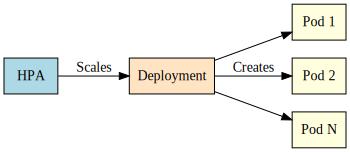
\includegraphics[width=1.0\textwidth]{hpa.png}
	\caption{HPA 控制器原理}
	\label{fig:hpa}
  \end{figure}
% \section{自定义自动伸缩系统}
% \subsection{系统的结构}
\section{流量模拟与伸缩实验}
\subsection{请求变化曲线的构造}

为了验证自动伸缩,首先需要生成流量的变化曲线。由于实际使用时伸缩的周期是
数小时,为了方便验证,我们将时间尺度缩小到数分钟。
然后,我们选用一个简单的函数来模拟请求流量的变化曲线。

具体而言,这个函数充当一个数据生成器,它可以根据给定的种子和长度,生成具有特定属性的
时间序列数据。我们希望这些数据具有一定的随机性,以模拟实际场景的不
确定性;同时,我们还希望它具有一定的周期性(包括短周期和长周期),以反映
某些周期性因素的影响;此外,我们希望这些数据具有整体的上升趋势,从而反映某些长
期趋势(例如业务增长)的影响。最后,我们希望这些数据是整数,并且其值在0~1000之间,
从而确保它们与实际的函数调用次数具有相同的数量级。

数据生成器函数的代码如下:

\begin{lstlisting}[language=Python]
import numpy as np
import matplotlib.pyplot as plt

def generate_data(seed, t_length, small_period=24, large_period=720):
    np.random.seed(seed)
    
    # 初始化序列
    y = np.zeros(t_length)
    
    # 生成随机步长。此处,我们使步长的平均值稍微偏正,以保证整体的升趋势。
    steps = np.random.randint(-40, 45, size=t_length - 1)
    
    # 计算随机漫步序列
    for t in range(1, t_length):
        y[t] = y[t-1] + steps[t-1]
        
    # 添加周期性趋势
    t = np.arange(t_length)
    y += np.sin(2 * np.pi * t / small_period) * 50  # 小周期趋势
    y += np.sin(2 * np.pi * t / large_period) * 100  # 大周期趋势,可以调整振幅以增加或减少周期性趋势的强度
    
    # 为了保证y的范围在0~1000之间,我们将y线性映射到这个范围
    y = (y - np.min(y)) / (np.max(y) - np.min(y)) * 1000
    
    # 因为y应该是整数,所以我们进行四舍五入
    y = np.round(y).astype(int)
    
    return y
\end{lstlisting}

它的工作原理如下:

首先,我们使用给定的种子初始化随机数生成器,以确保本研究的数据生成过程是可复
现的。然后,我们生成一个随机步长序列,这个步长序列可以是正的或负的,但
我们使其平均值稍微偏正,以保证整体的上升趋势。然后,我们使用这个步长
序列生成一个随机漫步序列,这个随机漫步序列体现了数据的随机性。

接下来,我们添加了两个周期性趋势。一个是小周期趋势,周期为24,模拟了一
天内的变化;另一个是大周期趋势,周期为720,模拟了一个月内的变化。我们使
用sine函数来生成这两个周期性趋势,因为sine函数是周期性的,而且它的值
在-1和1之间,这使得可以通过调整振幅来控制周期性趋势的强度。

最后,为了保证生成的数据的值在0~1000之间且是整数,我们将随机漫
步序列和周期性趋势的和线性映射到这个范围,然后进行四舍五入。线性映射
的过程是通过计算最小值和最大值,然后使用这两个值将数据缩放和平移到
目标范围。

\begin{figure}[htbp]
	\centering
	\includegraphics[width=1.0\textwidth]{images/generated_data.png}
	\caption{生成的数据示例}
	\label{fig:generated_data}
  \end{figure}

生成的数据的示例如图 \ref{fig:generated_data} 所示。

\subsection{基于模拟流量的自动伸缩仿真}

我们使用 0 到 999 时刻的数据作为初始历史数据,输入到 ARIMA 模型训练,
并预测 1000 时刻的访问量。从 1000 时刻开始,每隔 30 秒,采用下一个时
刻的数据点作为模拟的请求数量。并滑动历史数据窗口,将新的数据点加入到模型训练
的历史数据集中,以模拟实际的工作负载预测过程。

基于预测访问量,使用请求/容器数量的比例(记作k)来计算需要扩容至的容器数量。
此处我们采用 k=100,也即每个容器每秒处理100个请求的假设。此假设仅用于演示,其取值不影响
预测性能或伸缩效率。在实际应用时,应当根据服务器配置情况测量得到此参数。

\begin{figure}[htbp]
	\centering
	\includegraphics[width=1.0\textwidth]{images/y_replica.png}
	\caption{访问量与副本数量}
	\label{fig:y_replica}
  \end{figure}

图 \ref{fig:y_replica} 展示访问量与副本数量的关系,即假设伸缩不消耗时间情况下副本的数量关系。

\subsection{仿真结果与结果分析}

使用上述结果进行仿真,对于预测区间 [1001,2000] ,ARIMA 模型得到的结果如图 \ref{fig:arima_simulation} 所示。
作为基准的 MA(WIN\_SIZE=3)模型得到的结果如图 \ref{fig:ma_simulation} 所示。
这两张图展示实际值(蓝色曲线)与预测值(绿色曲线)之间的关系,同时使用右侧坐标轴
展示实际所需副本数和预测所需副本数之间的关系。

\begin{figure}[htbp]
	\centering
	\includegraphics[width=1.0\textwidth]{images/arima_simulation.png}
	\caption{ARIMA 模型仿真结果}
	\label{fig:arima_simulation}
  \end{figure}

  \begin{figure}[htbp]
	\centering
	\includegraphics[width=1.0\textwidth]{images/ma_simulation.png}
	\caption{MA 模型仿真结果}
	\label{fig:ma_simulation}
  \end{figure}

  表 \ref*{table:sim_regression_metrics} 展示模型的性能指标
  。从 MAPE、SMAPE 的结果来看,模型的预测性能较好。且 ARIMA 模型的性能在所有指标
  上超过 MA 模型。
  
  \begin{table}[tbp]
  \centering
  \caption{基于仿真数据预测的模型性能}
  \label{table:sim_regression_metrics}
  \begin{tabular}{c|c|c}
  \hline
  \textbf{指标} & \textbf{数值} & \textbf{MA 模型基准}\\
  \hline
  MSE & 169.09 & 243.23\\
  RMSE & 13.00 &  15.60\\
  MAE & 10.68 & 12.72\\
  MAPE & 5.78 \% &  6.89\%\\
  SMAPE & 5.78 \% & 6.87\%\\
  \hline
  \end{tabular}
  \end{table}

  而副本数量预测任务,由于相当于对访问量预测进行向上取整,预测的性能表现更为优异,
  如表 \ref{table:sim_classification_metrics} 所示。
  副本数量的预测几乎完全准确。且 ARIMA 模型的性能在所有指标
  上均优于 MA 模型。

\begin{table}[tbp]
	\centering
	\caption{基于仿真数据预测的模型性能(副本数量)}
	\label{table:sim_classification_metrics}
	\begin{tabular}{c|c|c}
	\hline
	\textbf{指标} & \textbf{数值} & \textbf{MA 模型基准}\\
	\hline
	MSE & 0.074 & 0.086\\
	RMSE & 0.27 & 0.29\\
	MAE & 0.074 & 0.086\\
	MAPE & 2.93 \% & 3.30\%\\
	SMAPE & 2.86 \% & 3.28\%\\
	\hline
	\end{tabular}
	\end{table}

\chapter{结论与展望}
\section{结论}
\subsection{本文的主要成果}
本研究中提出并实施了一种基于负载预测的 Serverless 计算的自动伸缩算法。主要发现如下:

\begin{itemize}
	\item 我们基于 MA、VAR、Prophet 和 ARIMA 模型实现了有效的流量预测机制,从而能够在工作负载发
	生变化之前做出响应,提前进行自动伸缩。通过对实际的 Serverless 工作负载进行实验,我们发现这些模型能够
	有效预测其变化趋势。
	
	\item 我们设计并实施了一套基于 Prometheus 的自动预警机制。通过收集 
	Serverless 应用的监控指标,并将这些数据输入到预测模型中,
	可以提前做出伸缩决策,从而避免因工作负载变化导致的性能下降或资源浪费。
	
	\item 我们还实现了函数副本数量的自动伸缩。通过调整副本数量,Serverless 应用可以
	根据实际的工作负载需求动态调整资源使用,从而提高资源利用率和运行稳定性。
\end{itemize}

值得一提的是,我们在每个预测时刻之前,会采用滑动窗口的方式重新训练模型,并且自动选择最优的 p,d,q 参数。
这主要有两点好处:一是可以避免历史数据膨胀导致预测的时间复杂度常数过高;
二是可以避免模型参数无法同步于历史数据的变化导致预测结果的不准确性。

\subsection{对实际问题的解决方案}
本研究所提出的自动伸缩算法和方案,为如何实现 Serverless 计算的自动伸缩提供了有效的解决方
案。通过自动预警、负载预测、自动伸缩的结合,可以在工作负载变化之前做出响应,动态调整函数副本
数量,提高资源利用率和运行稳定性。

\section{局限性与未来工作}
\subsection{本文的不足之处}
虽然本研究取得了一些重要的发现,但还存在以下不足之处:

\begin{itemize}
	\item 本研究的负载预测模型基于历史数据进行预测,但对于那些历史数据不足,预测准确性可能会降低。
	
	\item 我们发现多数的 Serverless 应用,即便在日尺度下有非常高的访问次数,但在分钟或秒的尺度
	之下,统计周期内可能根本没有访问,所以对于实际场景,精确到秒的预测的难度会非常大。这也是我们
	选择以小时为单位的原因。

	\item 允许零副本的情况下,本研究的自动伸缩算法由于采用向上取整,最少的副本数量为 1,这可能会导致资源浪费。

	\item 我们实验时发现特定时间点负载的变化幅度较大,导致频繁的伸缩行为,这可能会影响应用的性能。

\end{itemize}

\subsection{可进一步探讨和优化的方向}
针对上述不足之处,未来的研究可以从以下方向进行:

\begin{itemize}
	\item \textbf{使用预训练模型进行预测。} 可以考虑使用 Transformer 等模型,在同类 Serverless
	应用上进行预训练,再使用具体的应用进行微调,以提高预测的准确性\cite{wu2020deep}。

	\item \textbf{增加更多的预测特征。} 目前主要针对时间和访问次数进行预测,未来可以考虑
	引入更多内部和外部的特征,例如,CPU 使用率,内存使用率,网络延迟等,以提高预测的准确性。
	不过这主要适用于多特征的预测模型。

	\item \textbf{考虑支持零副本的缩容。} 对于重要度不高,能接受数秒的启动延迟的应用,
	可以考虑支持零副本的缩容,从而避免资源浪费。

	\item \textbf{考虑增加对临界值的特殊处理。} 预测值量变临界情况下,可以增加一定的迟滞性,从而避免
	过于频繁的伸缩。

\end{itemize}
这些方向将为我们提供更深入的理解和优化 Serverless 计算的自动伸缩。


%%%%%%%%%%%%%%%%%%%%%%%%%%%%% Main Area %%%%%%%%%%%%%%%%%%%%%%%%%%%%
%%%%%%%%%%%%%%%%%%%%%%%%%%%%% Main Area %%%%%%%%%%%%%%%%%%%%%%%%%%%%
%%%%%%%%%%%%%%%%%%%%%%%%%%%%% Main Area %%%%%%%%%%%%%%%%%%%%%%%%%%%%
%%%%%%%%%%%%%%%%%%%%%%%%%%%%% Main Area %%%%%%%%%%%%%%%%%%%%%%%%%%%%
%%%%%%%%%%%%%%%%%%%%%%%%%%%%% Main Area %%%%%%%%%%%%%%%%%%%%%%%%%%%%
%%%%%%%%%%%%%%%%%%%%%%%%%%%%% Main Area %%%%%%%%%%%%%%%%%%%%%%%%%%%%
 
%%%%%%%%%%%%%%%%%%%%%%% Main Area ENDs Here %%%%%%%%%%%%%%%%%%%%%%%%
%\let\cleardoublepage=\cleardoublepagebak

\begin{nopagenumber}
% Reference
\clearpage\phantomsection\addcontentsline{toc}{chapter}{参考文献}
\bibliographystyle{buptbachelor}
\refbodyfont{\bibliography{ref}}

% Thanks to page
\clearpage
\chapter{致\qquad{}谢}
\normalsize\thankwords

% Appendix
\setcounter{figure}{0} 
\renewcommand{\thefigure}{~附-\arabic{figure}~}
\setcounter{equation}{0} 
\renewcommand{\theequation}{~附-\arabic{equation}~}
\setcounter{table}{0} 
\renewcommand{\thetable}{~附-\arabic{table}~}
\setcounter{lstlisting}{0} 
\makeatletter
  \renewcommand \thelstlisting
       {附-\@arabic\c@lstlisting}
\makeatother




% Translated Article
\newpage\backmatter
\thispagestyle{empty}
\phantomsection\addcontentsline{toc}{chapter}{外\quad{}文\quad{}资\quad{}料}
% 原文第一页,PDF缩放比例为0.95,可以自行调整
\includepdf[pages=1, scale=0.95, pagecommand=\begin{center}\translationtitlefont{外\quad{}文\quad{}资\quad{}料}\end{center}]{docs/translation.pdf}
% 原文剩余部分
\includepdf[pages=2-, scale=0.95]{docs/translation.pdf}

% Translation
\setcounter{chapter}{0}
\renewcommand{\thefigure}{~外\arabic{chapter}-\arabic{figure}~}
\renewcommand{\theequation}{~外\arabic{chapter}-\arabic{equation}~}
\renewcommand{\thetable}{~外\arabic{chapter}-\arabic{table}~}
\renewcommand{\thelstlisting}{~外\arabic{chapter}-\arabic{lstlisting}~}

\begin{center}
\phantomsection\addcontentsline{toc}{chapter}{外\quad{}文\quad{}译\quad{}文}
\translationtitlefont{外\quad{}文\quad{}译\quad{}文}
\end{center}
\vspace{8mm}
\thispagestyle{empty}


\begin{center}
	\sanhao\heiti\textbf{深度Transformer模型在时间序列预测中的应用:流感盛行病例研究}

\xiaosihao\songti{Neo Wu, Bradley Green, Xue Ben, Shawn O'Banion}

\end{center}

\songti{}
\begingroup % 限制两个let语句的作用范围在外文译文部分
\let\clearpage\relax
\let\cleardoublepage\relax

%以下是排版示例,在此处为了使章节编号不出现在目录中,选用无编号的样式,代价是这些数字都要自己书写。
\section{摘要}
本文提出了一种新的时间序列预测方法。
在这篇文章中,我们提出了一种全新的时间序列预测技术。众所周知,时间序列数据在
许多科学和工程领域中都有广泛的应用。解读这些数据,并对其进行有效预测,一直是
机器学习领域中的一个核心问题。我们的研究团队开发了一种新颖的方法,该方法采用了
基于Transformer的机器学习模型
,目的就是提高我们对时间序列数据的预测精度。这个方法利用自注意力机制,从时间
序列数据中学习并理解其内在的复杂模式和动态变化。值得一提的是,这种预测框架具有很
高的通用性。不论是对单变量还是多变量的时间序列数据,或者是时间序列嵌入,都可
以应用这个框架进行预测。
为了验证这个新方法的有效性,我们进行了一项案例研究,选择了流感样似症(ILI)的
预测作为案例。研究结果表明,我们的方法所产生的预测结果与当前最先进的预测技术相比
,具有极高的竞争力。
\section{引言}
季节性流感的全球流行给我们的健康和经济带来了沉重的压力。据统计,全球每年因流
感致死的人数惊人地高达291,000至646,000人。在美国,疾病控制与预防中心(CDC)
会利用他们的监测网络,每周发布一次有关流感症状的报告。虽然这种方式在追踪疾病流
行的规模上发挥了重要作用,但由于数据收集和整理的时间,这些报告通常至少会有一周
的延迟。因此,预测流感症状的活动就显得尤为重要,它能够帮助我们实时监测疾病的
发展,以及为公共卫生机构分配资源、制定应对潜在大流行的计划和准备提供重要参考。

为了预测这些流感症状的时间序列数据,科学家们已经开发了各式各样的方法,从机械模
型到统计和机器学习的方法,应有尽有。其中,机械模型主要是基于对疾病传播动态的
理解。例如,像SIR这样的隔室方法就是常用的模拟疾病传播动态的工具。

统计和机器学习的方法则是借助真实数据去学习和掌握趋势与模式。其中,有一些广为流
传的方法,例如自回归(AR)、自回归滑动平均(ARMA)以及自回归积分滑动平均
(ARIMA)。除此之外,一些基于卷积和循环神经网络的深度学习方法也被开发出来
,用于模拟流感症状数据。这些序列对齐的模型自然是处理时间序列数据的首选。然而,
循环神经网络中存在梯度消失和梯度爆炸的问题,而卷积滤波器也有其局限性,这些都使得
这些方法在处理序列数据中的长期和复杂关系时有所不足。

在我们的这项研究中,我们基于Transformer架构开发了一种新颖的时间序列预测方法
。与序列对齐模型不同,Transformer并不是按照顺序处理数据,而是一次性处理整个
数据序列,并利用自我注意力机制去学习序列中的依赖关系。因此,基于Transformer
的模型具有一定的潜力,能够处理那些对于序列模型具有挑战性的复杂时间序列数据。我们以流
感症状预测为案例,展示了基于Transformer的模型在时间序列预测任务上的应用,
结果表明,这种模型优于许多现有的预测技术。

\begin{figure*}
    \includegraphics[width=\textwidth]{transformer_architecture.pdf}
    \caption{基于Transformer的预测模型架构}
  \end{figure*}
  
  \section{相关工作}
  一些研究使用互联网数据,如Google Trends、Twitter和Wikipedia来预测流感样似症比例。
  Google流感趋势(GFT)采用线性模型,利用预定义术语的Google搜索量来估计当前的流感样似症比例(“即时预测”)。
  尽管最初被认为是巨大的成功,但GFT在随后的几年中高估了峰值流感样似症数量。
  
  其他研究将GFT与新的建模技术和额外信号结合起来。
  Lazer等人提出了一种基于自回归(AR)的方法来扩展GFT。
  Santillana等人通过开发一种自动选择查询和更新流感样似症预测模型的模型,改进了GFT。
  Araz等人使用GFT数据和额外信号构建线性回归模型。
  Yang等人开发了一种基于自回归的模型,利用Google搜索数据(“ARGO”)来估计流感流行病。
  ARGO优于先前基于Google搜索的模型。
  最近,基于ARGO开发了一种新的集成模型(“ARGONet”)。
  这种新方法利用空间信息改进了模型,并实现了流感样似症预测的最新成果。
  
  深度学习技术也被用于流感样似症预测。
  Liu等人使用Google Trends、气候、空气污染和病毒学监测数据训练了基于LSTM的模型来预测流感流行程度。
  Venna等人开发了一个基于LSTM的多阶段模型,结合气候和时空调整因素进行流感预测。
  注意力机制也被应用于流感样似症预测。
  Zhu等人开发了多通道LSTM神经网络,可以从不同类型的输入中进行学习。
  他们的模型使用注意力层将模型输出与输入序列关联起来,进一步提高了预测的准确性。
  Kondo等人将序列到序列(“Seq2Seq”)模型与类似的注意力机制相结合,用于预测流感流行程度,并表明他们的方法优于ARIMA和基于LSTM的模型。
    
  \section{背景}
  \subsection{流感和流感样似症(ILI)}
  流感是一种由流感病毒感染引起的常见传染病。每年流感影响多达3500万人,给健康和经济带来巨大负担。在美国,疾病控制与预防中心(CDC)在一个广阔的地理区域内协调一个报告网络。网络中的参与健康提供者报告显示流感样似症(ILI)症状的患者统计数据。ILI症状通常定义为“发烧和咳嗽和/或喉咙痛”。ILI比例被计算为患有ILI症状的患者数量与当周总门诊人数的比值。CDC发布了美国和除佛罗里达州外的所有个别州的ILI比例。此外,州级的ILI比例还经过了对州人口的归一化处理。
  
  \subsection{状态空间模型}
  状态空间模型(State Space Models,SSM)广泛应用于动态系统。动态系统的演变受到不可观测的状态变量的控制。系统展现出由状态变量决定的可观测变量。SSM已应用于生物学和金融等复杂系统的研究中。
  
  状态空间模型同时建模状态变量和可观测变量。
  例如,广义线性状态空间模型可以用以下方程表示:
\begin{align}
x_t &= Z_t\alpha_t + \epsilon_t  \label{obs:eqn} \\
\alpha_{t+1} &= T_t\alpha_t + R_t\eta_t,  t = 1, ..., n, \label{state:eqn}
\end{align}
其中,$x_t$和$\alpha_t$分别是时间索引的观测向量和状态向量。
方程~\ref{obs:eqn}称为观测方程,它类似于回归方程。
它建模了可观测变量$x_t$与潜在状态变量$\alpha_t$之间的关系。
方程~\ref{state:eqn}是状态方程,具有自回归性质。
它控制了状态变量随时间的演变。
$\epsilon_t$和$\eta_t$是创新项,通常被建模为高斯过程。
在这一节中,我们简要提及了一些在ILI预测中常用的SSM模型。

\paragraph*{隔室模型}
隔室模型是SSM的一种特定形式,广泛应用于研究传染病。在隔室模型中,将人群分为不同的组(“隔室”)。每个组通过一个时间相关的状态变量来建模。一个著名的隔室模型是“易感-感染-康复”(Suscepted-Infected-Recovered,SIR)模型,该模型通过以下常微分方程来描述系统的演变:
\begin{align*}
\frac{dS}{dt} &= -\frac{\beta IS}{N}\\
\frac{dI}{dt} &= \frac{\beta IS}{N} - \gamma I\\
\frac{dR}{dt} &= -\gamma I
\end{align*}
在这个模型中,ILI时间序列是系统的可观测变量:$\mathrm{ILI}(t) = I(t) / (I(t) + S(t) + R(t))$。
尽管最初是为了建模传染病而开发的,隔室模型已被应用于生态学和经济学等其他学科。
虽然隔室模型很有用,但它们需要对微分方程的参数具有先验知识,并且缺乏在新观测数据下更新参数的灵活性。
    \paragraph*{ARIMA}
Box-Jenkins ARIMA(自自回归差分移动平均)是另一种常用的建模动态系统的方法。ARIMA模型对观测变量$x_t$进行建模,假设$x_t$可以分解为趋势、季节性和随机的成分。Box和Jenkins的想法是对时间序列$x_t$进行差分操作,以消除趋势和季节性。得到的序列被视为平稳时间序列数据,并使用其滞后时间序列值的组合(“AR”)和滞后预测误差的移动平均值(“MA”)进行建模。ARIMA模型通常由一个元组$(p, d, q)$来指定,其中$p$和$q$定义了AR和MA的阶数,$d$指定了差分操作的阶数。

ARIMA可以用SSM形式来表示,常见的SSM技术如滤波和平滑也可以应用于ARIMA。然而,ARIMA是一种“黑盒”方法,模型完全依赖于观测数据,没有对潜在系统状态的分析。

\paragraph*{时间延迟嵌入}
对于标量时间序列数据$x_t$,其时间延迟嵌入(TDE)是通过将每个标量值$x_t$嵌入到$d$维的时间延迟空间中形成的:
\begin{equation*}
\mathrm{TDE_{d, \tau}}(x_t) = (x_t, x_{t-\tau}, ..., x_{t-(d-1)\tau}) % TODO(neowu) check if whether this the right definition?
\end{equation*}
对于任何非线性动力系统而言,延迟嵌入定理(Takens定理)表明存在某个$(d, \tau)$-时间延迟嵌入,可以通过观测变量的延迟坐标近似恢复出原始状态变量(即“相空间”)的演化。在流感样似症预测的情况下,Takens定理表明通过对ILI比例(即“观测变量”)构造的$\mathrm{TDE_{d, \tau}}$,可以近似描述由生物学和物理机制控制的潜在动力系统。

Sugihara和May在开创性工作中首次探索了TDE在时间序列预测中的应用。他们展示了TDE可以通过对系统动力学的定性评估,无需了解底层机制,实现短期预测。他们开发了基于TDE的模型来预测水痘和麻疹的发病率,并将其与基于AR的方法进行比较。他们的分析表明,对于水痘病例的预测,TDE模型与AR模型表现相当,而对于麻疹病例的预测,TDE模型优于AR模型。

在状态空间模型(SSM)框架中,时间延迟嵌入是一种强大的工具,可以通过学习底层动力系统的几何和拓扑信息,将状态变量和观测数据联系起来,而无需理解系统的状态变量和相空间。尽管TDE具有令人惊叹的特性,但据我们所知,TDE在机器学习模型中尚未得到广泛研究。

\subsection{序列模型}
许多现实世界的机器学习任务涉及不同类型的序列数据,包括自然语言文本、音频和视频、DNA序列和时间序列数据。序列模型专门用于建模这种数据。在本节中,我们简要回顾几种常见的序列模型。

\paragraph*{循环神经网络}
与传统的前馈网络不同,循环神经网络(Recurrent Neural Networks,RNN)具有循环性质 - 它对每个输入$x_t$执行相同的函数,并且输出$y_t$依赖于输入$x_t$和前一个状态$h_{t-1}$。

\begin{figure}
\centering
\includegraphics[width=16cm,height=10cm,keepaspectratio]{rnn.pdf}
\caption{循环神经网络的折叠和展开表示}
\label{fig:rnn}
\end{figure}

如图~\ref{fig:rnn}所示,简单的循环神经网络(Simple RNN)可以表示为:
\begin{align*}
h_t &= \sigma(W_x x_t + W_h h_{t-1} + b_h) \\
y_t &= \sigma(W_y h_t + b_y)
\end{align*}
其中,$x_t$是输入向量,$h_t$是隐藏状态向量,$y_t$是输出向量。$W$和$b$是学习参数,$\sigma$是激活函数。

\paragraph*{长短期记忆网络(LSTM)}
虽然循环神经网络具有处理序列数据的内部记忆,但在处理长序列时会出现梯度消失和爆炸的问题。为了解决这个限制,专门开发了长短期记忆(Long Short-Term Memory,LSTM)网络。LSTM使用三个门,包括输入门、遗忘门和输出门,来调节细胞之间的信息流动,防止梯度消失和爆炸。

\begin{figure}
\centering
\includegraphics[width=16cm,height=10cm,keepaspectratio]{lstm.pdf}
\caption{长短期记忆网络和LSTM单元}
\end{figure}
\begin{align*}
f_t &= \sigma(W_f [h_{t-1}, x_t] + b_f) \\
i_t &= \sigma(W_i [h_{t-1}, x_t] + b_i) \\
\tilde{C_t} &= \tanh(W_C [h_{t-1}, x_t] + b_C) \\
C_t &= f_t * C_{t-1} + i_t * \tilde{C_t} \\
y_t &= \sigma(W_y [h_{t-1}, x_t] + b_y) \\
h_t &= y_t * \tanh(C_t)
\end{align*}
\paragraph*{序列到序列模型(Seq2Seq)}
序列到序列(Sequence-to-Sequence,Seq2Seq)架构是为了处理输入和输出都是序列的机器学习任务而开发的。Seq2Seq模型由三个组件组成,包括编码器(Encoder)、中间向量(Intermediate Vector)和解码器(Decoder)。编码器是一堆LSTM或其他循环单元。每个单元接收输入序列中的一个元素。编码器的最终隐藏状态被称为编码器向量或上下文向量,它编码了输入数据的所有信息。解码器也由一堆循环单元组成,并以编码器向量作为其第一个隐藏状态。每个循环单元计算自己的隐藏状态并产生一个输出元素。图~\ref{fig:seq2seq}展示了Seq2Seq架构。

Seq2Seq在语言翻译任务中得到了广泛应用。然而,它在处理长句子时性能下降,因为它无法充分将长序列编码到中间向量中(即使使用LSTM单元)。因此,在编码器向量中往往会丢失长期依赖关系。

\begin{figure}
\centering
\includegraphics[width=12cm,height=6cm,keepaspectratio]{seq2seq.pdf}
\caption{序列到序列模型架构}
\label{fig:seq2seq}
\end{figure}
    
    
    \section{模型}
    \subsection{问题描述}
    我们将ILI预测问题建模为一个监督机器学习任务。给定包含$N$个周数据点的时间序列${x_{t-N+1}, ..., x_{t-1}, x_t}$,对于$M$步预测,监督机器学习模型的输入$X$为${x_{t-N+1}, ..., x_{t-M}}$,输出$Y$为${x_{t-M+1}, x_{t-M+2}, ..., x_t}$。每个数据点$x_t$可以是一个标量或包含多个特征的向量。
 
    \subsection{数据}
我们利用了来自CDC的2010年至2018年的国家和州级历史ILI数据。

为了生成带标签的数据集,我们采用了固定长度的滑动时间窗口方法(图~\ref{fig:sliding-window}),构建用于模型训练和评估的${X, Y}$对。在应用滑动窗口之前,我们对所有数据进行最大最小值缩放,使用训练数据集的最大和最小值。然后在缩放后的训练集上运行滑动窗口,获得具有特征和标签的训练样本,其中特征是前N个观测值,标签是后M个观测值。测试样本也以相同的方式构建,用于模型评估。训练和测试集的划分比例为2:1。来自不同州的训练数据被连接起来形成全局模型的训练集。

\begin{figure}
\centering
\includegraphics[width=16cm,height=10cm,keepaspectratio]{sliding_window.pdf}
\caption{使用滑动时间窗口构建训练样本和测试样本}
\label{fig:sliding-window}
\end{figure}
    
    \subsection{Transformer模型}
    \subsubsection{模型架构}
    我们基于原始的Transformer架构构建了基于Transformer的ILI预测模型,包括编码器和解码器层。
    
    \paragraph*{编码器}
    编码器由输入层、位置编码层和四个相同的编码器层组成。
    输入层通过一个全连接网络将输入的时间序列数据映射为一个维度为$d_{\text{model}}$的向量。这一步对于模型使用多头注意力机制至关重要。
    使用正弦和余弦函数的位置编码对时间序列数据中的顺序信息进行编码,通过将输入向量与位置编码向量进行逐元素相加来实现。
    得到的向量被馈送到四个编码器层。每个编码器层包括两个子层:自注意力子层和全连接前馈子层。每个子层之后都有一个归一化层。
    编码器产生一个$d_{\text{model}}$维的向量,用于馈送给解码器。

\paragraph*{解码器}
我们采用了与原始Transformer架构相似的解码器设计。
解码器由输入层、四个相同的解码器层和一个输出层组成。
解码器的输入从编码器输入的最后一个数据点开始。
输入层将解码器输入映射为一个维度为$d_{\text{model}}$的向量。
除了每个编码器层中的两个子层外,解码器还插入第三个子层,对编码器输出应用自注意力机制。
最后,有一个输出层将最后一个解码器层的输出映射到目标时间序列。
在解码器中,我们采用前瞻遮挡和解码器输入与目标输出之间的一位偏移,以确保对时间序列数据点的预测仅依赖于先前的数据点。

\subsubsection{训练}
\paragraph*{训练数据和批处理}
在典型的训练设置中,我们训练模型从过去10个周的数据预测未来4周的ILI比例。
也就是说,给定编码器输入$(x_1, x_2, ..., x_{10})$和解码器输入$(x_{10}, ..., x_{13})$,解码器的目标是输出$(x_{11}, ..., x_{14})$。
我们使用前瞻遮挡来确保模型只会在目标数据之前的数据点上应用注意力。
也就是说,在预测目标$(x_{11}, x_{12})$时,遮挡确保注意力权重仅作用在$(x_{10}, x_{11})$上,以防止解码器从解码器输入中泄露关于$x_{12}$和$x_{13}$的信息。
训练时使用大小为64的小批量数据。
\paragraph*{优化器}
我们使用Adam优化器,其中$\beta_1 = 0.9$,$\beta_2 = 0.98$,$\epsilon = 10^{-9}$。
我们使用自定义的学习率和以下调度表进行训练:
\begin{align*}
lrate = &d_{\text{model}}^{0.5} * \min(\text{step\_num}^{0.5},\\
        &\text{step\_num} * \text{warmup\_steps}^{-1.5})
\end{align*}
其中$\text{warmup\_steps} = 5000$。

\paragraph*{正则化}
我们对编码器和解码器中的三种子层(自注意力子层、前馈子层和归一化子层)都应用了dropout技术。
每个子层的dropout率为0.2。

\subsubsection{评估}
在评估中,我们使用固定长度的滑动窗口构建了带有标签的测试数据。
经过训练的Transformer模型进行一步预测。
我们计算实际数据${y_i}$和预测值${\hat{y_i}}$之间的皮尔逊相关系数和均方根误差(RMSE)进行评估。
\subsection{ARIMA、LSTM和Seq2Seq模型}
本节介绍了我们开发的其他模型,用于对比Transformer-based模型的性能。

\paragraph*{ARIMA}
我们使用ARIMA模型作为基准模型。ARIMA模型将时变的ILI比例视为一个遵循固定动态的单变量时间序列。每周的ILI比例取决于前$p$周的观测值和前$q$周的估计误差。我们使用赤池信息准则(AIC)和贝叶斯信息准则(BIC)来选择ARIMA模型的阶数,以在模型复杂性和泛化性之间取得平衡。我们选择了$\mathrm{ARIMA}(3,0,3)$的阶数,并添加了一个常数趋势,以保持模型的简洁性。该模型基于状态空间建模框架进行训练,使用数据集的前三分之二进行训练。然后,使用拟合的参数对完整的时间序列进行滤波,进行四步的预测。

\paragraph*{LSTM}
LSTM模型由两个LSTM层的堆叠和一个最后的全连接层组成,直接预测多步的ILI比例。LSTM层通过循环网络从输入中编码顺序信息。全连接层接收来自第二个LSTM层的最终输出,并输出一个大小为4的向量,与预测的步数相对应。两个LSTM层分别具有32个和16个单元。为了正则化,我们在LSTM层中应用了0.2的丢弃率。训练时使用Huber损失、Adam优化器和学习率为0.02。

\paragraph*{Seq2Seq}
Seq2Seq模型采用了一种与Transformer模型类似的编码器-解码器架构,不过它并没有使用自注意力机制。它的编码器和解码器都由两层LSTM构成。编码器的作用是将输入的序列转化为一个上下文向量,然后解码器利用这个上下文向量以及前一个输出逐步生成目标序列。在训练这个Seq2Seq模型的过程中,我们采用了Huber损失、Adam优化器和0.02的学习率。

Seq2Seq模型的主要用途是作为基准模型,用来与基于Transformer的模型进行对比和性能评估。

\paragraph*{Seq2Seq}
我们测试的Seq2Seq模型也采用了编码器-解码器架构,编码器部分由一个全连接的稠密层
和一个GRU(门控循环单元)层组成,其主要任务是从输入的序列中提取和学习特征,最
终返回一组编码的输出和最后一个隐藏状态。解码器的结构设计与编码器部分基本相同
。在这个模型中,稠密层包含16个单元,而GRU层则包含32个单元。值得一提的是,这
个Seq2Seq模型还巧妙地融入了注意力机制。具体来说,解码器在每一步的解码过程
,都会利用Bahdanau注意力机制处理编码器的输出序列,以便更好地进行下一步的预
测。解码器还使用了一种名为“Teacher forcing”的技术,这有助于模型更快地收敛
,同时解决了不稳定性问题。这种技术的基本思路是,在训练过程中,我们会将当前时
间步的真实ILI比例作为下一个时间步的输入,而不是使用解码器单元计算出的输出。
此外,为了防止过拟合,所有的循环层中都采用了0.2的丢弃率。在训练这个模型的过
程中,我们使用了Huber损失函数、Adam优化器和0.02的学习率。
\section{实验}
\subsection{仅使用ILI数据进行一步预测}
\begin{figure*}
\includegraphics[width=\textwidth]{argo_transformer_corr.pdf}
\caption{ARGONet和Transformer模型的皮尔逊相关系数}
\label{fig:argo_transformer_corr}
\end{figure*}
\begin{figure*}
    \includegraphics[width=\textwidth]{argo_transformer_rmse.pdf}
    \caption{ARGONet和Transformer模型的均方根误差(RMSE)}
    \label{fig:argo_transformer_rmse}
    \end{figure*}
    
    在我们的第一个实验中,我们测试了我们基于Transformer的模型是否能够从历史数据中预测一周后的ILI比例。为了评估模型,训练好的全局模型使用测试数据集进行一步预测。计算了每个州的皮尔逊相关系数和均方根误差(RMSE)。
    
    我们将Transformer模型的性能与ARIMA、LSTM和带有注意力机制的Seq2Seq模型进行
    了比较。表~\ref{table:exp_compare}总结了每种方法的相关系数和RMSE,以及相
    对于ARIMA方法的性能提升。比较表明,深度学习模型在相关系数和RMSE方面整体优于
    ARIMA。在这三种深度学习方法中,相关系数非常接近,Transformer模型略高于
    LSTM和带有注意力机制的Seq2Seq模型。在RMSE方面,Transformer模型的
    性能优于LSTM和带有注意力机制的Seq2Seq模型,相对的RMSE减小分别为27%和8.4%
    。这个分析表明,注意力机制对预测性能起到了贡献,因为带有注意力机制的Seq2Seq
    和Transformer模型优于纯LSTM模型。此外,与带有注意力机制的Seq2Seq模型相
    比,Transformer模型显示出更好的预测性能,这表明Transformer的自注意机
    制能够更好地捕捉数据中的复杂动态模式。值得注意的是,Transformer在美国的
    ILI预测中显示出最佳的指标(皮尔逊相关系数=0.984,RMSE=0.3318)。由
    于单个模型使用来自所有州的数据进行训练,这表明该模型确实能够推广各个州
    的模式,用于国家级的预测。
    
    \begin{table}[h!]
        \centering
           \caption{模型性能总结及相对于基准模型的变化}
           \label{table:exp_compare}
           \begin{tabular}{| c || c | c ||}
           \hline
           模型 & 皮尔逊相关系数 & RMSE \\ [0.5ex]
           \hline\hline
           ARIMA &
             \begin{tabular}{@{}c@{}}0.769 \\ \small{(+0 \%)} \end{tabular} &
             \begin{tabular}{@{}c@{}} 1.020 \\ \small{(-0 \%)} \end{tabular}\\
             \hline
           LSTM &
             \begin{tabular}{@{}c@{}}0.924 \\ \small{(+19.9 \%)} \end{tabular} &
             \begin{tabular}{@{}c@{}} 0.807 \\ \small{(-20.9 \%)} \end{tabular}\\
             \hline
           Seq2Seq+注意力机制 &
             \begin{tabular}{@{}c@{}}0.920 \\ \small{(+19.5 \%)} \end{tabular} &
             \begin{tabular}{@{}c@{}} 0.642 \\ \small{(-37.1 \%)} \end{tabular}\\
             \hline
           Transformer &
             \begin{tabular}{@{}c@{}}0.928 \\ \small{(+20.7 \%)} \end{tabular} &
             \begin{tabular}{@{}c@{}} 0.588 \\ \small{(-42.4 \%)} \end{tabular} \\
             \hline
           \end{tabular}
        \end{table}
        \subsection{使用特征向量的逐步预测}
        接下来,我们测试了基于Transformer的模型是否能够从多个特征(即多变量时间序列数据)中学习进行ILI预测。
        在美国,流感季节通常从10月初开始,并在1月和2月之间达到高峰。
        我们假设周数是模型的一个信息量丰富的信号。
        因此,我们将“周数”作为一个与时间相关的特征引入模型中。
        此外,我们还在模型中包括时间序列的一阶和二阶差分作为两个显式的数值特征。

        我们的结果表明,包含这些特征可以提高模型的性能(平均皮尔逊相关系数:0.931,平均RMSE = 0.585)。
        然而,与仅使用ILI数据的Transformer模型相比,改进并不显著。
        这表明这些额外的特征可能对模型提供了较少的新信息。
        也就是说,如果基于Transformer的模型能够依赖自注意力机制从ILI时间序列中学习短期和长期依赖关系,那么引入的一阶和二阶差分特征很可能是多余的。
        
        我们将结果与ARGONet的ILI预测数据进行了比较,ARGONet是文献中的一种先进的ILI预测模型。
        图~\ref{fig:argo_transformer_corr}和图~\ref{fig:argo_transformer_rmse}显示了ARGONet和我们的Transformer模型的相关系数和RMSE值。
        总体而言,基于Transformer的模型与ARGONet的性能相当,平均相关系数略有改善(ARGONet: 0.912,Transformer: 0.931),平均RMSE值略有下降(ARGONet: 0.550,Transformer: 0.593)。
        
        \subsection{采用时间延迟嵌入法进行预测分析}

        在这一部分,我们针对基于Transformer的模型能否直接对动力系统的相空间进行建模进行了一番实验探究。我们采用了历史的ILI数据,以此构建出时间延迟嵌入(TDEs)。值得注意的是,当TDEs的维度足够多时,它在拓扑结构上就能等同于那些未知的动力系统相空间。
        
        换句话说,相对于我们观测到的标量变量ILI数据,TDEs所编码的内容包含了更丰富的几何和拓扑信息,这些信息是控制流感感染和传播过程的系统必需的。因此,如果我们采用TDEs,就能获取到比标量时间序列输入更丰富的信息。
        
        为了检验这个理论,我们从ILI数据中构建了从2到32维的时间延迟嵌入,并以此作为特征,进行基于Transformer的ILI预测。在表\ref{tde:dim}中,我们列出了在不同TDE维度$d$下的预测指标结果。在所有的实验中,我们均采用了$\tau=1$来构建TDEs。
        
        通过观察我们发现,改变TDE的维度并不会对皮尔逊相关系数产生显著影响。然而,在维度增加的过程中,RMSE值先是降低,后又趋于稳定,其中在维度为8时达到了最小值。这个结果与预测水痘和麻疹所使用的最优TDE维度相近,那时的最优维度分别为5和5-7。
        \begin{table}[h!]
            \centering
            \caption{时间延迟嵌入的性能}
            \label{tde:dim}
            \begin{tabular}{| c || c | c ||}
            \hline
            维度 & 皮尔逊相关系数 & RMSE\\ [0.5ex]
            \hline\hline
            2 & 0.926 & 0.745 \\ [1ex]
            \hline
            4 & 0.929 & 0.778 \\ [1ex]
            \hline
            6 & 0.927 & 0.618 \\ [1ex]
            \hline
            8 & 0.926  & 0.605  \\ [1ex]
            \hline
            16 & 0.925 & 0.623 \\ [1ex]
            \hline
            32 & 0.925 & 0.804 \\ [1ex]
            \hline
            \end{tabular}
            \end{table}
            
            \section{结论}
            在这项研究里,我们提出了一种全新的,基于Transformer的时间序列预测技术。相比其他依赖于序列对齐的深度学习方法,我们的方法可以更有效地利用自注意力机制来捕捉和模拟序列数据的特性,从而能在时间序列数据中学习并理解各种长度和复杂度的依赖关系。

            值得一提的是,我们所采用的基于Transformer的方法构成了一个通用框架,能够处理和建模各种非线性动力系统。这一点在ILI案例中得到了清晰的展示:这种方法能够通过时间延迟嵌入来建模观察到的时间序列数据和状态变量的相空间。此外,这种方法还具备较强的可扩展性,无论是对单变量还是多变量的时间序列数据建模,都只需对模型实现进行微小的修改即可。
            
            最后,我们想要强调的是,尽管目前的案例研究主要集中在时间序列数据上,我们坚信我们的方法有着更广泛的应用潜力,可以进一步扩展到建模以时间和位置坐标为索引的时空数据。这是因为自注意力机制有着极强的泛化能力,可以用来学习时空空间中任意两点之间的关系。这也将是我们未来研究的重要方向。

\endgroup

% 开题报告
\blankmatter
\phantomsection\addcontentsline{toc}{chapter}{开\quad{}题\quad{}报\quad{}告}
\includepdf[pages=-]{docs/openingReport.pdf}

% 中期检查表
\blankmatter
\phantomsection\addcontentsline{toc}{chapter}{中\quad{}期\quad{}检\quad{}查\quad{}表}
\includepdf[pages=-]{docs/interimReport.pdf}

% 教师指导毕业设计(论文)记录表
\blankmatter
\phantomsection\addcontentsline{toc}{chapter}{教师指导毕业设计(论文)记录表}
\includepdf[pages=-]{docs/guidance.pdf}

\end{nopagenumber}

\end{document}
